\documentclass[10pt,a4paper,twoside]{article}
\usepackage[top=1.5in,bottom=1in,left=1.125in,right=1.125in]{geometry}
\usepackage{amsmath}
\usepackage{amssymb}
\usepackage{amsthm}
\usepackage[center]{caption}
\usepackage{booktabs}
\usepackage{xcolor}
\usepackage{enumitem}
\usepackage{fancyhdr}
\usepackage{graphicx}
\usepackage{latexsym}
\usepackage{lipsum}
\usepackage{longtable}
\usepackage{multirow}
\usepackage{multicol}
\usepackage{tasks}
\usepackage[singlespacing]{setspace}
\usepackage[ngerman]{babel}
\usepackage{wrapfig}
\usepackage{pgfplots}

% Biblatex
\usepackage{csquotes}
\usepackage[
    backend=biber,
    style=numeric,
    natbib=true,
    sorting=none,
    block=nbpar,
    backref=true
]{biblatex}
\addbibresource{lib/bib.bib}
\usepackage{hyperref}

% If you want to break on URL numbers
\setcounter{biburlnumpenalty}{9000}
% If you want to break on URL lower case letters
\setcounter{biburllcpenalty}{9000}
% If you want to break on URL UPPER CASE letters
\setcounter{biburlucpenalty}{9000}

\pagestyle{myheadings}
% \setlength{\parindent}{0.8in}

\usepackage{float}

% Graph--------------------------------------------------------------------------------------------
\usepackage{graphics,graphicx}
\usepackage{calc}
\usepackage{tikz}
\usetikzlibrary{decorations.markings}
\tikzstyle{vertex}=[circle, draw, inner sep=2pt, minimum size=4pt]
\newcommand{\vertex}{\node[vertex]}
\newcounter{Angle}

\renewcommand{\baselinestretch}{1.25}

% ???
\newcommand*{\QEDA}{\hfill\ensuremath{\large{\lozenge}}}
\newcommand*{\QEDAa}{\hfill\ensuremath{\square}}

% Centering table of contents and list of table
% \usepackage{tocloft}
% \renewcommand{\contentsname}{\hfill\bfseries\Large Inhaltsverzeichnis \hfill}
% \renewcommand{\cftaftertoctitle}{\hfill}

\usepackage{titletoc} % for mutli toc's
\usepackage[explicit]{titlesec}
\setcounter{secnumdepth}{3}
\setcounter{tocdepth}{3}

\definecolor{DarkGreen}{RGB}{3,103,16}
\renewcommand{\thefootnote}{\textcolor{DarkGreen}{\arabic{footnote}}}

\usepackage[bottom]{footmisc}

% Variablen ---------------------------------------------------------------------------------------
    \newcommand{\autorFirstNameT}{Tim}
    \newcommand{\autorFirstNameK}{Konstantin}
    \newcommand{\autorFamilyNameT}{Kretzschmar}
    \newcommand{\autorFamilyNameK}{Blechschmidt}
    % Kürzere Referenzierung
% Variablen ---------------------------------------------------------------------------------------

% Eigenschaften einstellen
\hypersetup{
    pdftitle={},
    pdfauthor={\autorFirstNameT \autorFirstNameK} {\autorFamilyNameT \autorFamilyNameK},
    pdfcreator={\autorFirstNameT \autorFirstNameK} {\autorFamilyNameT \autorFamilyNameK},
    pdfkeywords={AmIVulnerable} {CVE} {Both} {\autorFamilyNameT} {\autorFamilyNameK},
    pdfnewwindow = true,
    colorlinks,
    pdfpagelabels,
    pdfstartview = FitH,
    bookmarksopen = true,
    bookmarksnumbered = true,
    linkcolor = black,
    urlcolor = blue,
    plainpages = false,
    hypertexnames = false,
    citecolor = blue
}

% Anhang
\usepackage[toc,page]{appendix}
\renewcommand\appendixname{Appendix}
\renewcommand\appendixpagename{Appendix}
\renewcommand\appendixtocname{Appendix}
% Abkürzungen
\usepackage{acronym}
\usepackage{tabularx}
\usepackage{ltablex}

\begin{document}
    \nocite{*}

    \phantomsection
    \addcontentsline{toc}{section}{Inhaltsverzeichnis}
    \tableofcontents\label{Inhaltsverzeichnis}

    \newpage

    % Lorem, ipsum dolor sit amet consectetur adipisicing elit. Molestias aut, repellat ipsum facere voluptate dicta obcaecati deserunt nobis suscipit eaque?
    % \begin{wrapfigure}{l}{0.5\textwidth}
    %     \centering
    %     \begin{tikzpicture}
    %         \begin{axis}[
    %             ybar,
    %             bar width=0.5cm,
    %             width=0.48\textwidth,
    %             height=6cm,
    %             ymin=0,
    %             xlabel={$x$},
    %             ylabel={Werte},
    %             xtick={1,2,3,4,5},
    %             xticklabels={1, 2, 3, 4, 5},
    %             xtick=data,
    %             nodes near coords,
    %             nodes near coords style={/pgf/number format/.cd,fixed zerofill,precision=1},
    %             nodes near coords align={vertical},
    %             ]
    %             \addplot coordinates {(1,1) (2,34) (3,23) (4,123) (5,84)};
    %             \addplot[smooth, red, mark=*] coordinates { 
    %                 (0, {(1 + 34 + 23 + 123 + 84) / 5})
    %                 (6, {(1 + 34 + 23 + 123 + 84) / 5})
    %             };
    %         \end{axis}
    %     \end{tikzpicture}
    %     \caption{Balkendiagramm}
    % \end{wrapfigure}
    % Lorem, ipsum dolor sit amet consectetur adipisicing elit. Molestias aut, repellat ipsum facere voluptate dicta obcaecati deserunt nobis suscipit eaque?
    % Lorem, ipsum dolor sit amet consectetur adipisicing elit. Molestias aut, repellat ipsum facere voluptate dicta obcaecati deserunt nobis suscipit eaque?
    % Lorem, ipsum dolor sit amet consectetur adipisicing elit. Molestias aut, repellat ipsum facere voluptate dicta obcaecati deserunt nobis suscipit eaque?
    % Lorem, ipsum dolor sit amet consectetur adipisicing elit. Molestias aut, repellat ipsum facere voluptate dicta obcaecati deserunt nobis suscipit eaque?
    % Lorem, ipsum dolor sit amet consectetur adipisicing elit. Molestias aut, repellat ipsum facere voluptate dicta obcaecati deserunt nobis suscipit eaque?
    % Lorem, ipsum dolor sit amet consectetur adipisicing elit. Molestias aut, repellat ipsum facere voluptate dicta obcaecati deserunt nobis suscipit eaque?
    % Lorem, ipsum dolor sit amet consectetur adipisicing elit. Molestias aut, repellat ipsum facere voluptate dicta obcaecati deserunt nobis suscipit eaque?
    % Lorem, ipsum dolor sit amet consectetur adipisicing elit. Molestias aut, repellat ipsum facere voluptate dicta obcaecati deserunt nobis suscipit eaque?

    \newpage

    \section{Abstract} \label{sec:abstract}
Das Entwickeln von Softwarelösungen ohne Bibliotheken, Frameworks oder externe Module ist heutzutage nicht mehr denkbar.
Abhängigkeiten bestimmen Funktionalität, Effizienz und Sicherheit der jeweiligen Softwarelösung und sind so ein sensibler Punkt der Softwareentwicklung.
Allerdings ist die Verwaltung dieser Abhängigkeiten mit ihren, teils transitiv vererbten, Sicherheitslücken mit steigender Zahl immer komplexer.
Um nun also eine fundierte Entscheidung über eine Abhängigkeit treffen zu können muss die mangelnde Transparenz der Abhängigkeitsstruktur von Softwarelösungen berichtigt werden.
\\
Diese Arbeit stellt die Entwicklung einer API vor, die es ermöglicht transitive Vererbungen von Abhängigkeiten darzustellen.
Laufzeitmessungen und Vergleiche durch diese mit anderen Tools zeigen die Effizienz und Wirksamkeit der entwickelten Lösung.
Ziel einer solchen Lösung ist es, das Verständnis und Management von Abhängigkeiten in der Softwareentwicklung zu verbessern, was letztendlich zu einer verbesserten Sicherheit und Effizienz von Softwarelösungen führen soll.
    \newpage
    \subsection{Motivation} \label{subsec:Motivation}
    Beim Entwickeln von Softwarelösungen gibt es viele Herausforderungen und Probleme. 
    Diese werden durch viele bereits vorhandene Softwarepakete bewältigt.
    Die Nutzung frei verfügbarer Softwarepakete sind deshalb im Arbeitsalltag gang und gäbe.
    Freiwillige oder Hobby-Programmierer ermöglichen mit ihrem Einsatz, dass weltweit die Entwicklung neuer Software sowohl im kommerziellen als auch privaten und öffentlichen Bereich vereinfacht, vereinheitlicht und beschleunigt wird.
    Dank der Konkurrenz freier Pakete, zum Beispiel anhand ihrer Nutzungszahl, gestaltet sich dort ein Wettbewerb, der gute Pakete beständig besser werden lässt und nicht durchdachte entweder (a) an Bedeutung verlieren lässt oder (b) soweit verbessert, dass ihre Funktionen und Benutzbarkeit anschließend überzeugen konnten.
    Ein anderer essentieller Aspekt außer der Nutzbarkeit oder Funktionserfüllung ist die Sicherheit.
    Eben jene muss sich bei jedem Paket separat und gekapselt gesehen auf einem solchem Niveau befinden, dass ihre Verwendung keine fahrlässig Gefahr darstellt.
    Dies beginnt bei zu kurzen Schlüssellängen und endet bei komplexen Programmen mit verschiedenen Angriffsschwachstellen.
    \\ \\
    Der Aufgabe Einschätzung der Sicherheit und Einhaltung von Standards hat sich die Mitre Corporation gestellt; eine us-amerikanische Forschungsabteilung der "National Cybersecurity FFRDC", die staatliche Finanzierung genießt.
    CVE nennt sich ihr Referenziersystem und stellt dabei die englische Abkürzung \glqq Common Vulnerabilities and Exposures\grqq~dar.
    \\
    Aber die Aufgabe, für jedes verwendete Paket einzeln die Sicherheitslücken nachzulesen oder für eine Paketsammlung nachzuvollziehen, ist selbst mit dem Angebot der \glqq National Cybersecurity FFRDC\grqq~zeitaufwendig und ressourcenintensiv - schließlich werden so personelle Kräfte und Rechenkapazitäten gebunden.
    Eine Automatisierung der Analyse solcher Pakete zielt somit nicht nur eine Reduktion des Zeitaufwandes mit sich, auch ist eine umfangreichere Analyse ohne Mehraufwand möglich.
    Dies spiegelt sich beispielsweise in der Möglichkeit wieder, ganze Projekte direkt analysieren zu lassen anstelle der einzelnen Pakete.
    \\
    Das zeigt, dass ein dringender Bedarf an einem Werkzeug besteht, das Entwicklern und Managern eine transparente und umfassende Analyse der Abhängigkeiten auf Sicherheitslücken bietet.
    Solch ein Werkzeug könnte einem Unternehmen weiterhin verschiedene Vorteile im Bereich der Softwareentwicklung für Transparenz, Qualität und Sicherheit bringen.
    \begin{enumerate}
        \item Transparenz und Vertrauen\\
            Durch eine klare Übersicht über genutzte externe Softwarekomponenten mit Sicherheitslücken können frühzeitig besser informierte Entscheidungen getroffen und potenzielle Risiken identifiziert werden.
        \item Qualität\\
            Entwickler können leichter erkennen, ob Abhängigkeiten ersetzt oder aktualisiert werden müssen.
        \item Sicherheit\\
            Um die Gesamtsicherheit einer Applikation bestmöglich zu gewährleisten trägt ein solches Tool, welches Schwachstellen und Abhängigkeiten auch in tieferen Ebenen von Abhängigkeiten darstellt, zur Identifikation und Vermeidung von Sicherheitslücken bei. 
    \end{enumerate}
    Insgesamt hilft ein solches Werkzeug bei der Entscheidungsfindung über externe Softwarekomponenten sowie bei der Aufdeckung von Sicherheitsrisiken.
    \newpage
    \section{Definitionen} \label{sec:Definitionen}
\begin{itemize}
    \item \textbf{CVE (Common Vulnerabilities and Exposures):} \\
    
    Der Aufgabe Einschätzung der Sicherheit und Einhaltung von Standards hat sich die Mitre Corporation gestellt; eine us-amerikanische Forschungsabteilung der "National Cybersecurity FFRDC", die staatliche Finanzierung genießt.
    CVE nennt sich ihr Referenziersystem und stellt dabei die englische Abkürzung \glqq Common Vulnerabilities and Exposures\grqq~dar.
    \\
    \glqq Common Vulnerabilities and Exposures\grqq~bzw. häufige Schwachstellen und Risiken sind als Liste öffentlich verfügbar.
    In dieser Liste werden nur die Schwachstellen betrachtet, die durch eine der 364 \glqq CVE Numbering Authority's\grqq (CNA's) eine CVE-Nummer zugewiesen bekommen haben.\cite{}
    Eine CVE-Nummer beinhaltet wiederum keine technischen Informationen zur Betroffenen Software- oder Hardwarekomponente sondern Produktname, Version, eine Beschreibung der Schwachstelle und gegebenenfalls werden Hinweise zur Behebung vermerkt.
    Diese Informationen müssen über andere Services oder Datenbanken, wie z.B. in der \glqq U.S. National Vulnerability Database\grqq~oder der \glqq CERT/CC Vulnerability Notes Database\grqq.

    \item \textbf{Direkte Abhängigkeiten:} \\
    In der Softwareentwicklung ist eine Abhängigkeit ein Softwarepaket, welches von der Anwendung selbst benötigt wird, um korrekt zu funktionieren.
    Diese Abhängigkeiten können direkt oder indirekt sein.
    Indirekte Abhängigkeiten sind solche, die durch andere Abhängigkeiten eingeführt werden.
    Direkte Abhängigkeiten sind typischerweise externe Softwarekomponenten oder Bibliotheken.
    Diese werden auch als Paket bezeichnet. 

    \item \textbf{Transitive Abhängigkeiten:} \\
    Transitive Abhängigkeiten sind indirekte Abhängigkeiten, die durch andere Abhängigkeiten benötigt werden.
    Wenn nun eine Applikation ein Paket einbindet welches ein weiteres Paket selbst benötigt, so ist dieses eine transitive Abhängigkeit der Applikation.
    Somit können sich rekursiv Abhängigkeitsbäume aufspannen, die teils sogar gleiche Pakete in verschiedenen Versionen einbinden.
    
    \item \textbf{API (Application Programming Interface):} \\
    Eine API definiert eine Reihe von Regeln und Mechanismen, über die verschiedene Softwarekomponenten miteinander interagieren können.
    Somit bieten stellen sie Schnittstelle zwischen verschiedenen Systemen dar.
    Sie legt fest, wie Softwaremodule oder -anwendungen miteinander kommunizieren, indem sie Funktionen, Methoden, Protokolle und Datenstrukturen bereitstellt.
    Um eine API zu nutzen müssen diese Festlegungen eingehalten werden.
    
    
    \item \textbf{JSON (JavaScript Object Notation):} \\
    JSON ist ein in der Webentwicklung verbreitetes Datenformat.
    Genutzt wird dieses um strukturierte Daten zu speichern und auszutauschen.
    Basierend auf einer einfachen Syntax, die auf Schlüssel-Wert-Paaren und verschachtelten Datenstrukturen basiert ermöglicht es für Mensch sowie Maschine eine gute Les- und Parsbarkeit.
    JSON wird häufig für die Übertragung von Daten zwischen Client und Server.
    Dabei ist es programmiersprachenunabhängig verwendet allerdings Konventionen ählnich der von C, C++ oder C\#.

    \item \textbf{Container:} \\
    \item \textbf{Kubernetes:} \\
    \item \textbf{CI/CD:} \\
\end{itemize}
    \newpage
    \section{Andere Arbeiten} \label{sec:Andere}
Vor der Konzeption der Softwarelösung einer Dependency-API muss erst ein Blick auf die bisherige Forschung und Entwicklung in diesem Bereich geworfen werden.
Es gibt bereits verschiedene Applikationen, API's und Plattformen, die sich mit der Herausforderung beschäftigen, Abhängigkeiten in Softwarelösungen zu verwalten und potenzielle Sicherheitsrisiken zu identifizieren.
Folgend werden einige der bekanntesten Softwarelösungen betrachtet, die für diese Zwecke entwickelt wurden.
Es soll ein Überblick über den aktuellen Stand der Technik und mögliche Herausforderungen entstehen um Herausforderungen, denen sich Entwickler bei der Verwaltung von Abhängigkeiten und der Gewährleistung der Sicherheit in ihren Projekten gegenübersehen, besser einzuschätzen.
\subsubsection{NIST-API} \label{subsubsec:NIST_API}
    NIST-API
\subsection{Github Dependa Bot} \label{sec:Dependa}

\subsubsection{Snyk} \label{sec:Snyk}
Die Synk Plattform ist ein weiteres Tool, mit welchem Sicherheitsschwachstellen in Applikationen gemanagt werden können.
Es werden betroffene Abhängigkeiten identifiziert und Lösungen angeboten diese Schwachstellen zu schließen.

Es werden verschiedene Teile der Softwareentwicklung von Synk betrachtet darunter der Code selbst, Container und die Infrastruktur.
\glqq Synk Open Source\grqq~erkennt Schwachstellen in \glqq Open Source\grqq-Abhängigkeiten und \glqq Synk Code\grqq~erkennt diese im Code selbst.
\glqq Synk Container\grqq~erkennt Schwachstellen in Container-Images sowie Kubernetesanwendungen.
\glqq Synk Infrastructure as Code (IaC)\grqq~erkennt Fehlkonfigurationen in Terraform, CloudFormation, Kubernetes und Azure-Formlagen.

Durch Synk werden nicht nur Meldungen generiert, welche Abhängigkeiten Schwachstellen aufweisen sondern in der gesammten Deployment-Kette auf Schwachstellen geachtet.
Lösungen bzw. Alternativen werden angeboten und zusätztlich kann dieses Tool auch in die CI/CD eingebunden werden um einen sicherheitskritischen Bau der Applikation zu verhindern.   
\subsubsection{OWASP Dependency-Check} \label{sec:OWASP-Dependency-Check}
    Das Software-Composition-Analysis-Tool Dependency Check von der OWASP Foundation analysiert die Codebasis auf bekannte Schwachstellen.
    Dabei werden auf Common-Platform-Enumeration-Kennungen (CPE) für die genutzten Abhängigkeiten geprüft und falls vorhanden ein Bericht mit zugehöriger \ac{CVE}-Nummer erstellt.

    Die durch die automatischen Analysen erstellten Berichte enthalten nicht nur die jeweiligen Schwachstelle selbst, sondern auch Maßnahmen zum Schließen jener.
    \newpage
    \section{Konzept} \label{sec:Konzept}
    Im Rahmen dieser Arbeit soll eine \ac{API} zur Verfügung gestellt werden, die es ermöglicht transitive Vererbungen von Abhängigkeiten darzustellen.
    Dabei sollen einzelne Pakete, Listen von Paketen und ganze Projekte selbst analysiert werden können.
    Abhängigkeiten werden durch Extraktion eines Abhängigkeitsbaumes erkannt und einzeln gegen Schwachstellendaten geprüft.
    Der Nutzer, bzw. Maschinen sollen letztendlich ein weiterverwendbares klares Datenformat erhalten in welchem betroffene Abhängigkeiten und Ihre Schwachstellen vermerkt sind.
    \subsection{Forschungsfragen} \label{sec:Forschungsfragen}
    Aus den funktionalen und nichtfunktionalen Anforderungen ergeben sich folgende Forschungsfragen für diese Arbeit:
    \\ \\
    Forschungsfrage \ref{q:one}, welche aus den funktionalen Anforderungen \ref{f:one} und \ref{f:two} hervorkommt, betrachtet die Analyse von einzelnen oder Listen von Abhängigkeiten auf Basis der eingeladenen Schwachstellendaten.
    Je nachdem, ob eine Menge an Abhängigkeiten oder eine Einzelne gesucht werden muss müssen hier verschiedene Algorithmen implementiert werden um eine effiziente Ergebnisfindung zu gestalten.
    \\ \\
    Forschungsfrage \ref{q:two} handelt von den zu implementierenden Funktionalitäten für Repositories und geschieht aufbauen auf Forschungsfrage \ref{q:one}.
    Deshalb sind die folgenden funktionalen Anforderungen \ref{f:one}, \ref{f:three}, \ref{f:four} und \ref{f:five} zu betrachten.
    Dazu muss zuerst betrachtet werden, welche Ausgangsdaten vorliegen.
    Zusätzlich auch die zu analysierenden Repositories bzw. Abhängigkeiten und die genutzten Schwachstellendaten.
    \\ \\
    Forschungsfrage \ref{q:three} definiert den Rückgabetyp der Daten.
    Vor allem die nichtfunktionale Anforderung \ref{nf:four}, der Rückgabe im JSON-LD-Format, ist Ausschlaggebend.
    Hier müssen demnach sinnvolle Rückgabedaten für den Endnutzer identifiziert sowie eine Definition dieser vorgenommen werden.
    \\ \\
    Forschungsfrage \ref{q:four} behandelt die Umsetung der API selbst.
    Es ist die Umsetzung der Funktionalen Anforderungen unter der Betrachtung der nicht funktionalen Anforderungen.
    Vor allem nichtfunktionale Anforderung \ref{nf:five}, die Nutzung von Etablierten Technologien, hat hier ihren Schwerpunkt.
    Hierfür wird eine Programmiersprache mit zugehörigem Framework ausgewählt sowie das Endpunktdokumentations- und Testmöglichkeitstool.
    Es muss sich in diesem Umfeld auch auf eine Programmiersprache im Sinne der zu untersuchenden Projekte entschieden werden um den Umfang dieser Arbeit möglichst genau zu halten.
    Der entstandene Service muss, wie durch funktionale Anforderung \ref{f:seven} bestimmt, weiterhin im Container-Kontext nutzbar sein.
    \\ \\
    Forschungsfrage \ref{q:five} beschäftigt sich mit der Optimierung der API.
    Funktionale Anforderung \ref{f:six} und nichtfunktionale Anforderungen \ref{nf:one}, \ref{nf:two} und teils auch \ref{nf:three} sind hier zugehörig.
    Hier müssen algorithmische sowie technologische Verbesserungen in Leistung oder Laufzeit aufgezeigt und mögliche Lösungswege aufgezeigt oder implementiert werden.
    Besonders gewählte Datenbankformate werden hier thematisiert.

    
    
    \newpage
    \subsection{Funktionale Anforderungen} \label{sec:Funktionale_Anforderungen}
    Bei der Umsetzung dieser Schwachstellenanalyse-\ac{API} ergeben sich nun verschiedene funktionale Anforderungen aus den Forschungsfragen:
    \begin{enumerate}[label=\textbf{FRQ-\Roman*}, leftmargin=2.5cm]
        \item Einladen und Konvertieren der Schwachstellendaten und persistente Speicherung dieser in einer internen Datenbank (betrifft \ref{q:one}, \ref{q:two})\label{f:one}
        \item Überprüfung von Paketen auf Sicherheitslücken mittels Abgleich zur internen Schwachstellendatenbank (betrifft \ref{q:one}) \label{f:two}
        \item Clonen eines Repositories über Git. (betrifft \ref{q:two}) \label{f:three}
        \item Überprüfung von allen Abhängigkeiten eines Repositories mittels Abgleich zur internen Schwachstellendatenbank (betrifft \ref{q:two}) \label{f:four}
        \item Extraktion und Rückgabe eines Abhängigkeitsbaums für alle Abhängigkeiten mit Sicherheits\-lücken (betrifft \ref{q:two}) \label{f:five}
        \item Aktualisierung der Schwachstellendaten-Basis (betrifft \ref{q:five}) \label{f:six}
        \item Bereitstellung der \ac{API} in einem Container (betrifft \ref{q:four}) \label{f:seven}
    \end{enumerate}
    Diese Funktionalitäten setzten teils mehrere interne Abläufe voraus und beinhalten mehrere Endpunkte der \ac{API}.

    \subsection{Nichtfunktionale Anforderungen} \label{sec:N_Anforderungen}
    Weiterhin ergeben sich der Umsetzung dieser \ac{API} aus den Forschungsfragen verschidene nichtunktionale Anforderungen:
    \begin{enumerate}[label=\textbf{NFRQ-\Roman*}, leftmargin=2.5cm]
        \item Die Suche eines einzelnen Pakets dauert nicht länger als 5ms (betrifft \ref{q:five}) \label{nf:one}
        \\
        Erläuterung:
        Die Dauer einer Antwort der API sollte 5 Sekunden nicht überschreiten.\textsuperscript{\cite{link:ApiResponseTime}}
        \\
        Appendix \ref{sec:PackageMeanPopGitJsRepos} weist nach, daß in den beliebtesten JavaScript-Repositories durchschnittlich $2`429.9$ Abhängigkeiten bestehen und somit maximal $\frac{5\text{ Sekunden}}{2`429.9}$ betragen sollte, was $0.002$ Sekunden, also 2 Millisekunden entspricht.
        \\
        Das ein Projekt jedoch solch hohe Anzahlen beinhaltet ist ebenfalls aus den Rohdaten der 10 Repositories nicht immer der Fall und somit wird für die Analyse mit $1'000$ Paketen gerechnet -- der Median der Reihe beträgt $788$ -- und es ermittelt sich daraus der Grenzwert $\frac{5\text{ Sekunden}}{1`000} = 5$ Millisekunden für die Suche eines einzelnen Paketes.
        \item Skalierbarkeit der Anwendung (betrifft \ref{q:five}) \label{nf:two}
        \item Dokumentation der Endpunkte (betrifft \ref{q:five}) \label{nf:three}
        \item Rückgabe der Daten im \acs{JSON-LD}-Format (betrifft \ref{q:three}) \label{nf:four}
        \item Nutzung passender, etablierter Technologien (betrifft \ref{q:four}) \label{nf:five}
    \end{enumerate}
    \subsection{Besondere Merkmale} \label{sec:Besondere Merkmale}
Dadurchm dass diese API bei schachstellenbefallenen Abhängigkeiten den Abhängigkeitsbaum darstelle ist für den Nutzer eine hohe Granularität und Transparenz der Abhängigkeit gegenüber gegeben.
Somit können Aufwand bei Ersatz oder Anpassung an dieser besser eingeschätzt und die Entscheidung der Dringlichkeit dieser Arbeiten besser gefällt werden.
\\ \\
Durch die große Menge an CVE-Daten, die als Schwachstellen-Suchbasis dient, und dadurch, dass diese Datenbasis immer nur erweitert wird ist der der API ermöglicht nur die aktuell neuesten Änderungen herunterzuladen und einzupflegen.
Damit ist es nicht notwendig bei jeglichen Aktualisierungen die gesamte Datenbasis ernuet herunterzuladen.
\\ \\
Durch die lokal vorliegende Datenbasis ist das Suchen auf dieser deutlich schneller als diese Daten immer erneut anzufragen.
Somit kann mit einer niedrigeren Laufzeit in z.B. CI/CD intergrationen dieser gerechnet werden als andere Tools.
    \subsection{Erwartete Ergebnisse} \label{sec:Erwartete Ergebnisse}
    Folgende Ergebnisse sind im Rahmen dieser Arbeit zu erreichen:
    \begin{enumerate}
        \item \textbf{Entwicklung einer funktionsfähigen API} \\
            Diese soll performant und möglichst schmal in einem Containercontext nutzbar sein und alle -- von den Features -- notwenigen Endpunkte beinhalten.
        \item \textbf{Analyse auf Sicherheitslücken} \\
            Die entstehende API soll Sicherheitslücken in Abhängigkeiten ausfindig machen und diese in einem weiterverwendbaren Format zurückliefern.
        \item \textbf{Darstellung der detektierten Schwachstellenpakete inklusive Abhängigkeiten als Baum} \\
            Bei Analyse eines Repositories sollen alle Abhängigkeiten dieses mit dessen Abhängigkeiten aufgezeigt werden.
        \item \textbf{Entscheidungsunterstützung bei Abhängigkeitsveränderungen} \\
            Die entstehende API soll dem Nutzer letztendlich dabei helfen, eine Entscheidung über das Weiterverwenden oder Austauschen bzw. Aktualisieren einer Abhängigkeit zu fällen.
    \end{enumerate}

    \subsubsection{Architektur V1} \label{sec:Architektur}
    Um eine API umzusetzen und diese zu nutzen sind verschiedene Komponenten nötig:
    \begin{enumerate}
        \item \textbf{Framework} \label{arch_1}\\
            Als API-Grundlage muss ein passendes Framework genutzt werden.
            Dadurch, dass keine Notwendigkeit für ein Frontend besteht gibt es hier wenig Eingrenzungen.
            \\ \\
            Aus Erfahrungsgründen wurde das C\# Framework ASP.NET gewählt.
            Mit diesem lassen sich unter anderem API-Services bauen.
            Mittels der für das .NET Framework expliziet vorhandenen IDE \glqq Visual Studio\grqq~bestehen auch native Debugging-Möglichkeiten.
            Durch die große und aktive Community von ASP.NET ist dieses Framework sehr gut dokumentiert und es existieren viele Open-Source-Bibliotheken.
        \item \textbf{Datenbank} \label{arch_2}\\
            In der Datenbank sind alle CVE-Daten zu persistieren, welche zu durchsuchen sind.
            Diese Daten dienen als Grundlage der Identifizierung von Schachstellen in Paketen innerhalb von Projekten.
            Wichtig sind hier schnelle Lesezugriffe, da diese beim Abfragen der Datenbank die größte Laufzeiteinsparung bringen.
            \\ \\
            Durch die Wahl des Frameworks auf ASP.NET ist es möglich einen \textit{embedded NoSQL-Document-Store} -- LiteDB zu nutzen. % TODO: https://www.litedb.org/
            Diese ist leicht intern nutzbar und muss nicht separat explizit gestartet und verwaltet werden, womit diese auch im Container der API mit enthalten ist.
        \item \textbf{Controller} \label{arch_3}\\
            Controller einer API nehmen HTTP-Anfragen entgegen und reagieren darauf.
            Hier wird die Hauptaufgabe der API geschehen, da alle Funktionalitäten, sei es Datenbankabfragen, Klonen eines zu untersuchenden Repositories oder die Untersuchung dieses, in einem solchen implementiert oder aufgerufen werden müssen.
            \\ \\
            Notwendig sind hier view Controller.
            Für die Forschungsfrage \ref{one} bzw. \ref{three} muss ein Git-Controller zum nutzen von CVE-Daten sowie zum Erhalt von zu analysierenden Repositories entstehen.
            In diesem sind Endpunkte zum clonen des CVE-Daten-Repositories sowie zum clonen des Analyse-Repositories zu implementieren. % TODO: clone CVE-DATEN-REPO-LINK
            \\
            Weiterhin ist ein Controller für Abhängigkeiten nötig, in dem man aus dem zu analysierenden Repositoriy den Abhängigkeitsbaum extrahiert sowie diesen mit Schwachstellendaten anreichert.
            \\
            Für die Untersuchung einzelner Pakete und Listen dieser ist ein weiterer Endpunkt zu implementieren.
            In diesem ist auch die Update-Funktion der Datenbasis hinzuzufügen.
            \\
            Für Forschungsfrage \ref{two} muss in jedem Endpunkt bei korrekter Antwort ein Context mitgeliefert werden, damit der gelieferte Inhalt so durch JSON-LD zu interpretieren ist.
            Weiterhin sind durch einen Controller die Rückgabedaten zu dokumentieren.
            Dazu ist zwischen Softwarepaketen und CVE-Einträgen zu unterscheiden.
        \item \textbf{Datenmodelle} \label{arch_4}\\
            Um Daten korrekt in die Datenbank einzufügen, um ein Resultat-JSON zu erzeugen oder die Paketliste intern zu verarbeiten -- dazu sind Datenmodelle nötig.
        \item \textbf{Konvertierung von und in JSON} \label{arch_5}\\
            Beim Einlesen der CVE-Daten in die Datenbank ist eine Konvertierung vom vorhandenen JSON-Format in Einträge der Datenbank vorzunehmen.  
            Die aus der Datenbank genutzten, durch den Controller verarbeiteten, Daten müssen nun schließlich im JSON-Format dem Benutzer übermittelt werden.
            \\ \\
            Dies muss in den jeweiligen Controllern geschehen.
            Damit die Daten besser weiterverwendbar sind muss zusätzlich ein Kontext \glqq @context\grqq~hinzugefügt werden.
        \item \textbf{Container} \\
            Um die API unabhängig von der Umgebung und möglichst Speicheraufwandsschmal zu nutzen muss die Anwendung \glqq Containerisiert\grqq~werden.
            \\ \\
            Für den bau der Containers wird Docker-Compose genutzt.
    \end{enumerate}

    \newpage
    \section{Implementation} \label{sec:Implementation}
Vor der Implementation ist die Entscheidung der Auswahl der Einzelkomponenten, welche im Abschnitt \ref{Architektur} vorgestellt wurden, zu treffen.
\\ \\
Zuerst ist die Programmiersprache sowie das genutzte Framework zu definieren.
Aus Erfahrungsgründen wurde das C\# Framework ASP.NET gewählt.
Mit diesem lassen sich unter anderem API-Services bauen.
ASP.NET hat mit Visual Studio auch direkt eine Entwicklungsumgebung sowie Debugging Möglichkeiten.
Weiterhin gibt es die Möglichkeit die eingebette NoSQL-Datenbak LiteDB zu nutzen.
Durch die große und aktive Community von ASP.NET ist dieses Framework sehr gut dokumentiert und es existieren viele Open-Source-Bibliotheken.
\\ \\
Es wurden weiterhin verschiedene Experimente vorgenommen um Teile der Architektur und deren Implementation durch verschiedene Softwarekomponenten zu Vergleichen.
\subsection{Experimente} \label{sec:Experimente}
    Aus der Forschungsfrage \ref{q:five} ergeben sich Experimente, die auf Skalierbarkeit und Laufzeit der API abziehlen.
    \subsubsection{LiteDB Pipeline} \label{sec:ExperimentePIPE}
    Um die Suche von mehreren Paketen in der Datenbasis zu beschleunigen wurde sich das Prinzip der Parallelisierung zu Nutzen gemacht.
    Hierzu wurde die zu untersuchende Liste von Paketen auf verschiedene Tasks aufgeteilt.
    So ist nach dem vollständigen Befüllen der Pipeline eine theoretischen Laufzeitverkürzung um der Faktor der maximal abarbeitbaren Tasks erreicht.  
    
    Dabei sind zwei Fälle zu unterscheiden:
    \begin{description}
        \item[\textit{Weniger} Pakete als Datenbank-Dateien]\hfill \\
            In diesem Falle einer geringeren Anzahl an Pakete wird die Pipe nie vollständig gefüllt.
        \item[\textit{Mehr} Pakete als Datenbank-Dateien]\hfill \\
            In jenem Falle muss die Paketliste Stück für Stück in die Pipe eingefügt werden und beim Erreichen der Kapazität -- entsprechend der Anzahl der Datenbanken -- das früheste Paket entfernt und ein neues Paket am Anfang eingefügt werden.
    \end{description}
    
    Die Verwaltung der 3 verschiedenen Staaten der Pipe ist in folgender Abbildung mit \ac{PAP} nachvollziehbar.
    Anschließend sind die 3 Fälle näher ausgeführt.
    \begin{figure}[H]
        \centering
        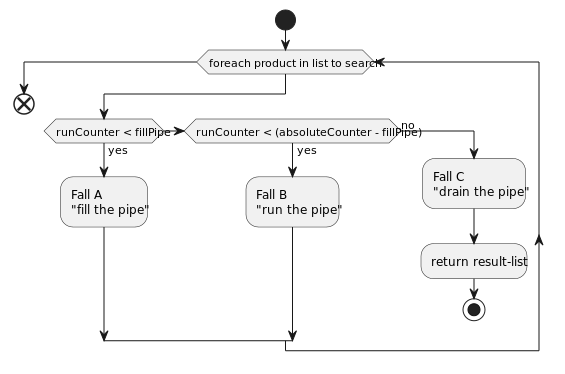
\includegraphics[width=\textwidth]{../pap/Simultanius search on LiteDb-Files.png}
        \caption{Übersicht der Pipeline-Staaten}
        \label{png:OverviewPipelineStatus}
    \end{figure}

    Das Befüllen der Pipeline geschieht nach folgendem Muster:
    \begin{figure}[H]
        \centering
        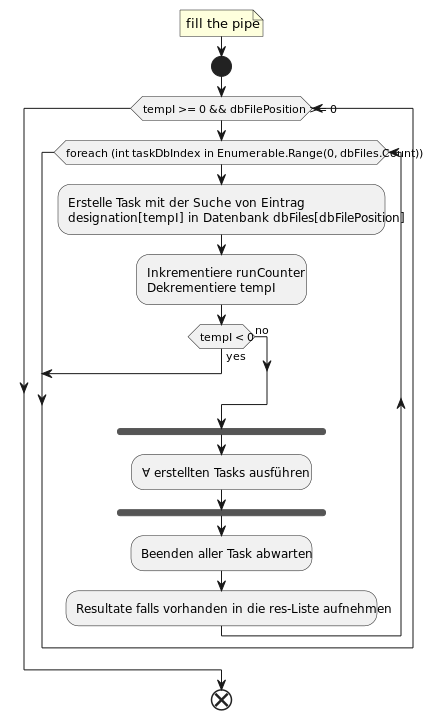
\includegraphics[width=\textwidth]{../pap/Case_A.png}
        \caption{\ac{PAP} Befüllen der Pipeline}
        \label{png:case_a}
    \end{figure}

    Nach vollständiger Befüllung die Erhaltung der Pipeline:
    \begin{figure}[H]
        \centering
        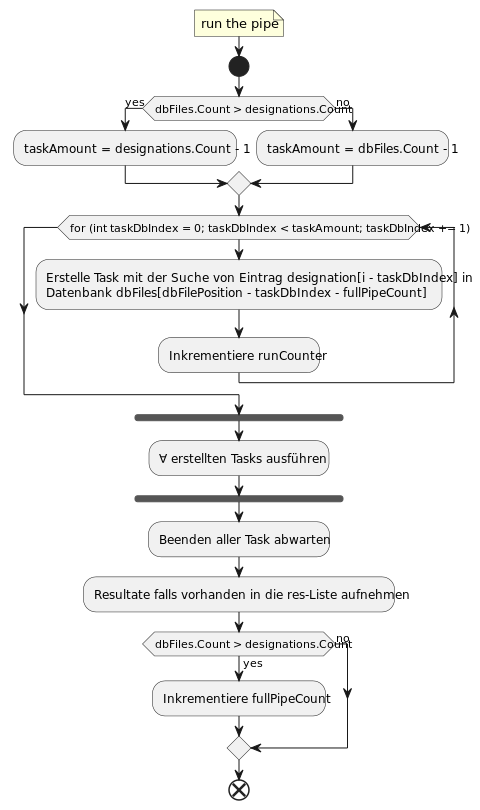
\includegraphics[width=\textwidth]{../pap/Case_B.png}
        \caption{\ac{PAP} Aufrechterhalten der Pipeline}
        \label{png:case_b}
    \end{figure}

    Beim Leeren der Pipeline:
    \begin{figure}[H]
        \centering
        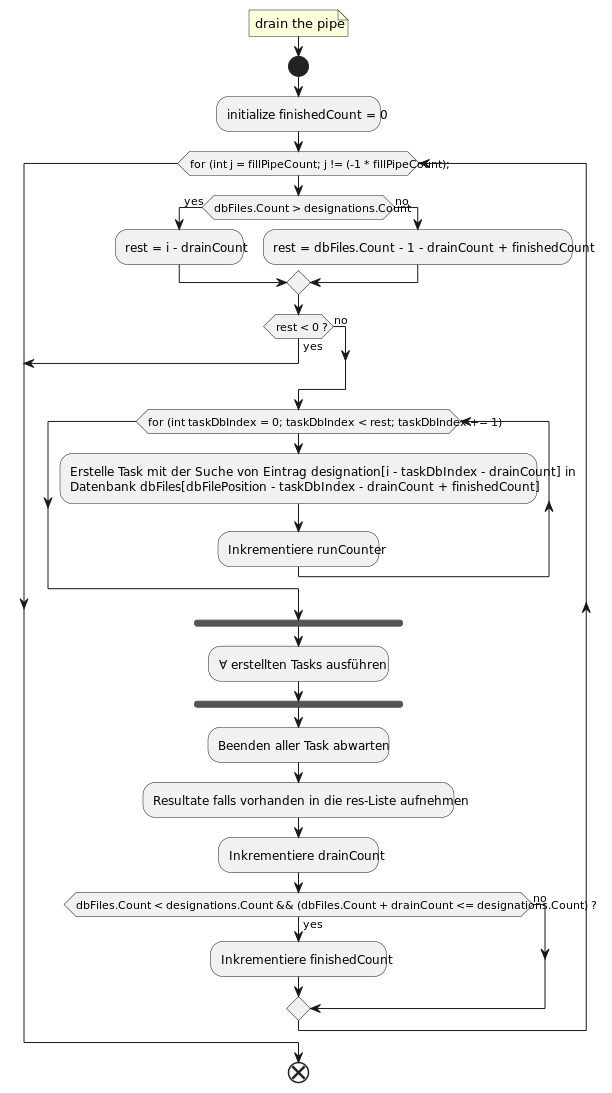
\includegraphics[width=\textwidth]{../pap/Case_C.png}
        \caption{\ac{PAP} Leeren der Pipeline}
        \label{png:case_c}
    \end{figure}

    Aus der Implementation der Pipeline ergeben sich folgende Laufzeiten bei weniger Paketen als Datenbankdateien:
    \begin{tabular}{|c|c|c|}
        \hline
            Such-Typ & Zeit & Faktor \\
            Mono-Suche & 262676.7ms & 1 \\
            Pipeline & 96868.4ms & 2.7213448 \\
        \hline
    \end{tabular}

    Aus der Implementation der Pipeline ergeben sich folgende Laufzeiten bei weniger Paketen als Datenbankdateien:
    \begin{tabular}{|c|c|c|}
        \hline
            Such-Typ & Zeit & Faktor \\
            Mono-Suche & 95011.24ms & 1 \\
            Pipeline & 22111.5ms & 4.296846569 \\
        \hline
    \end{tabular}

    \subsubsection{Datenbank} \label{sec:Experimente}
Die Wahl der Datenbank hat einen großen Einfluss auf die Laufzeit von Anfragen auf diese.
Aus der Gegebenen Einbindung einer NoSQL Datenbanklösung in ASP.NET, LiteDB, wurde diese auch zuerst als Datenspeicher gewählt.
\\
--> reicht diese Begründung für die Entscheidung? \\

Wieso Entscheidung auf Änderung? \\

Vergleich Messwerte (Am besten Messreihen) in Tabelle auf welchen Datenmengen? \\

--> Entscheidung auf welche DB am Ende, weil? \\
--> Einsparung von was am Ende? \\
    \subsubsection{MySQL Indexierung} \label{sec:MySQL_Indexierung}
    Die expliziten gemessenen Differenzen zwischen der Suche auf einer und der selben Tabelle einmal mit und einmal ohne erzeugten Index kann im Appendix unter \ref{subsec:MySQLMitIndex} \& \ref{subsec:MySQLOhneIndex} eingesehen werden.
    \\
    Eine Indizierung auf einer Tabelle in MySQL erzeugt Bereiche auf der Spalte, mit denen die Suche sehr beschleunigt werden.
    Laut der offiziellen Webseite von MySQL ist ohne Index die Suche auf einer Tabelle sequenziell von oben nach unten.\textsuperscript{\cite{link:MySqlIndex}}
    Dagegen ermöglicht die Suche mit einem erstellten Index der Datenbank, schon beim ersten Tabellenzugriff lediglich einen Bereich von Datensätzen zu durchsuchen.
    Damit sollte die Leistung merklich verbessert werden.
    \\
    Nachfolgend die arithmetische Mittel aus jeweils 10 Messungen auf der selben Tabelle mit und ohne Index:
    \\
    \begin{tabularx}{0.8\textwidth}{|c|c|c|}
        \hline
        Such-Typ & Zeit & Faktor \\ \hline
        ohne Index & 207,86ms & 1 \\
        mit Index & 0,710666667ms & 292,48593 \\
        \hline
        \caption{Laufzeiten Durchschnitt 10 Messungen \textsuperscript{siehe Appendix \ref{subsec:MySQLMitIndex} \& \ref{subsec:MySQLOhneIndex}}}
        \label{tabularx:MySqlIndexWithAndWithout}
    \end{tabularx}

    %!!!! SUCHE AUF JSON VS DB FILE
    Experimente
    \begin{itemize}
        \item Laufzeitmessungen LiteDB (Mono vs. Pipe -- schon schneller, aber nicht genug $\rightarrow$ fragments/searchStatistics.md)
        \item conclusio geht es schneller mit einer relationalen Datenbank?
    \end{itemize}
    \newpage
    % \section{Verifikation} \label{sec:Verifikation}

    % \newpage
    \section{Diskussion} \label{sec:Diskussion}

    \newpage
    \section{Zusammenfassung} \label{sec:Zusammenfassung}
    Die in der \nameref{subsec:Motivation} aufgelisteten Forschungsfragen können wie folgt nach Bearbeitung des Auftrages beantwortet werden:
    \begin{description}
        \item[\ref{q:one}]\hfill \\
            Um die Pakete zu untersuchen ist es notwendig, die \ac{CVE}-Daten in eine interne Datenbank umzuwandeln, da das Suchen auf den Rohdaten -- den \ac{CVE}-\ac{JSON}-Dateien -- zu zeitaufwendig ist.
            Dazu wurde schlussendlich eine MySQL-Datenbank ausgewählt, die dank der Indizierung einer Spalte die gewünschten Leistungsmerkmale aufweist.
        \item[\ref{q:two}]\hfill \\
            In der umgesetzten Version ist es dank der nativen Unterstützung von npm gelungen, die Abhängigkeiten der Pakte als \ac{JSON} zu extrahieren und dann intern so weiterzuverarbeiten, dass eine logische Repräsentation erfolgen kann.
        \item[\ref{q:three}]\hfill \\
            Die Lösung dieser Frage geschah über die einheitliche Verwendung von \ac{JSON} respektive \linebreak[4] \ac{JSON-LD} bei der Rückgabe des Webservices.
        \item[\ref{q:four}]\hfill \\
            Da die Aufgabe darin bestand, Github-Repositories zu analysieren, konnte in den Docker-Container der \ac{API} git mitinstalliert werden, wodurch ein voller Zugriff der \ac{API} auf den Funktionsumfang von git besteht.
            Durch diesen erlangte die \ac{API} die Möglichkeit Repositories zu clonen und anschließend intern weiterzuverarbeiten, was den Funktionsumfang der selbst-implementierten Methoden aus den Punkten $I$ bis $III$ der Forschungsfragen bereits entsprang.
        \item[\ref{q:five}]\hfill \\
            Die Frage nach der Laufzeitverbesserung stellte sich nach der Umsetzung der V1 (näheres in \ref{sec:Implementation1}), da dort die Wartezeiten für die Abfrage von Paketen den zeitlichen Rahmen übertraf.
            Nach der Umsetzung einer Pipeline zur Verbesserung der Laufzeit überbot man jedoch ebenfalls die selbstgesetzt zeitliche Beschränkung der Suche eines Paketes an sich.
            \\
            Die Überwindung der Zeitmauer gelang dann durch die in der V2 (\ref{sec:Implementation2}) verwendeten anderen Datenbank -- dann MySQL.
    \end{description}
    Erstmals war es gelungen einen Webservice zu implementieren, welcher ein Repository auf Schwachstellen untersucht, anstatt nur einzelne Pakete auf Treffer in Schwachstellendatenbanken zu über\-prüfen.
    Unsere Arbeit konnte nachweisen, dass eine solche Implementierung nach genannter \linebreak[4] Architektur -- \ref{sec:ArchitekturV1} -- möglich und die Hauptfunktion einer Rückgabe eines Abhängigkeitsbaumes, angereichert mit Schwachstellendaten, erfüllt ist.
    \\ \\
    Basierend auf dieser Arbeit sehen wir die Forschungsfragen
    \begin{itemize}
        \item \glqq \textit{Wie sind Schwachstellen auf Versions- und Commitbasis verteilt}\grqq,
        \item \glqq \textit{Wie gestaltet sich die Schwachstellenverteilung in verschiedenen Projekttypen, Frameworks oder Sprachen}\grqq$~$und
        \item \glqq \textit{Untersuchung von mehrfach vorkommenden Schwachstellen durch gleiche Abhängigkeiten beziehungsweise verschiedene Versionen dieser}\grqq
    \end{itemize}
    als besonders wichtig an.
    Da jene maßgeblich als Grundlage die Ergebnisse dieser Arbeit darstellen, um dem Endbenutzer eine einerseits fundierte und andererseits messbare Entscheidungsunterstützung im Verlauf eines Projektes beziehungsweise bei einem Refactoring zu bieten.
    \\
    Weitere mögliche Erweiterungen -- besprochen im Abschnitt \ref{sec:Diskussion} \nameref{sec:Diskussion} -- sind aufbauend und benötigen keine konkreten Änderungen in dem Grundgerüst, welches mit dem vorliegendem Projekt erreicht wurde.
    \\ \\
    Der zu dem Zeitpunkt der Abgabe aktuelle commit im Github-Repository wie folgt getagt: \\
    \href{https://github.com/WSE-research/AmIVulnerable/releases/tag/v2.0}{github.com/WSE-research/AmIVulnerable/releases/tag/v2.0}
 

    % \section{Einleitung} \label{sec:Einleitung}
    (1)
    als sub sections:\\
    Problemstellung
    Motivation
    Vorgehen (zur Lösung)
    % \section{Recherche} \label{sec:Recherche}
    \subsection{CVE} \label{subsec:CVE}
CVE, oder Common Vulnerabilities and Exposures \cite{}
    \subsection{Umgang mit CVE} \label{subsec:Umgang_mit_CVE}
Umgang mit CVE
    \subsection{Referenzen} \label{subsec:Referenzen}
    Referenzen und \ac{CVE}-Nutzungen
    \subsubsection{NIST-API} \label{subsubsec:NIST_API}
    NIST-API
    \subsubsection{DEPENDA-BOT} \label{subsubsec:DEPENDA_BOT}
    DEPENDA-BOT (GITHUB)
    \subsubsection{Weitere} \label{subsubsec:Weitere}
    Weitere
    % \section{Umsetzung} \label{sec:Umsetzung}
    (3)
    (sub)
    Technologiestack
        ASP.NET
        DOCKER
        LiteDB (NOSQL) erst
        MySQL (SQL) Ausblick
    API
        Modells
            PUML (Klassen)
            Interaktion und Zusammenhang der Klassen/Fktn
        Controller
            Auflistung und Erklärung (Swagger screenshot) in Paragraphs
            Views (JSON-LD def von CVE-Result, JSON-LD von NodePackageResult)
        DB-Anbindung: LiteDB braucht DB-Controller
        
    % \section{Analyse} \label{sec:Analyse}
    (4)
    (sub)
    Laufzeitmessungen nach Datenbankerstellung (etwa 1 std rechnen)
        JSON-Datei Suche VS LiteDB suche (60 min vs 8 s): Rechnung nach wie vielen Suchanfragen sich das ganze gelohnt hat (nach etwa einer)
    Laufzeitanalyse Mono-Suche und Pipeline-Suche auf LiteDB
        Wie ist LiteDB-Suche zu verschnellern
        Vergleich der Messungen
        Erklärung der Pipeline (Diagramme) (Wie und Warum, LiteDB ist File-Basier und deswegen kann auf mehreren Dateien gesucht werden falls genug threads zur verfügung stehen)
    Ausblick
        Ziel: schneller als NIST API sein (so und so viele Sekunden übers Netz im vergleich zu so und so vielen sekunden über unsere API)
        Um Ziel zu erreichen: Andere Datenbank verwenden um Lesezugriffe optimieren

    % \section{Conclusion} \label{sec:Conclusion}
    \subsection{Vision} \label{subsec:Vision}
Vision
    Validieren ob Ziel erreicht ist, dass
        ein Node-JS-Projekt komplett analysisert (alle Pakete entnommen werden) und nach Schwachstellen untersucht werden
        das zurückgegebene Format der API sinnvoll und struckturiert ist
        Wurde sich an programmiertechnische Standards gehalten
            Models sind eigene Bibliothek (losgelöst von der API, können weiterverwendet werden getrennt und weiterentwickelt werden)
            Controller liegen im Controller-Namespace
            Sinnvolle Trennung von Endpunkten in Controller mit http-Signatur
            Routennamen der Endpunkte in natürlicher Sprache/Pfaden
    \input{subsections/nächste_schritte.tex}
            

    \newpage
    \begin{appendices}
        \section{Abkürzungen} \label{sec:Abkürzungen}
    \begin{acronym}[LangesWortFuerDieEinstellung]
        \acro{API}[API]{\textbf{A}pplication \textbf{P}rogramming \textbf{I}nterface}
        \acro{NIST}[NIST]{\textbf{N}ational \textbf{I}nstitute for \textbf{S}tandards and \textbf{T}echnology}
        \acro{CVE}[CVE]{\textbf{C}ommon \textbf{V}ulnerabilities and \textbf{E}xposures}
        \acro{CNA}[CNA]{\textbf{C}VE \textbf{N}umbering \textbf{A}uthority}
        \acro{JSON}[JSON]{\textbf{J}ava\textbf{S}cript \textbf{O}bject \textbf{N}otation}
        \acro{JSON-LD}[JSON-LD]{\textbf{J}ava\textbf{S}cript \textbf{O}bject \textbf{N}otation \textbf{L}inked \textbf{D}ata}
        \acro{PAP}[PAP]{\textbf{P}rogramm \textbf{A}blauf-\textbf{P}lan}
    \end{acronym}
        \newpage
        \section{Messungen} \label{sec:Messungen}
            \startcontents[Messungen]
            \printcontents[Messungen]{}{2}{} % \printcontents[⟨name⟩]{⟨prefix⟩}{⟨start-level⟩}[⟨toc-depth⟩]{⟨toc-code⟩}
            \subsection{Zeitunterschied Abfrage auf den Datenbanken Mono-Pipe -- Fall: weniger Pakete als Datenbanken} \label{subsec:ZeitunterschiedAbfrageAufDenDatenbankenMonoPipeFallWenigerPaketeAlsDatenbanken}
    \subsubsection{Messung 1 von 10} \label{subsubsec:LiteDbWenigerPaketeAlsDb1von10}
        {\shorthandoff{"}
            {\small
                \begin{tabularx}{\textwidth}{|l|l|X|}
                    \hline
                    \textbf{Zeitstempel} & \textbf{Typ} & \textbf{Nachricht} \\
                    \hline
                    \endhead
                    2024-02-20 16:52:48.970 +01:00 & [INF] & Time by mono LiteDB completed in 4147.1 ms \\
                    2024-02-20 16:52:51.848 +01:00 & [INF] & Time by mono Newtonsoft completed in 2866.1 ms \\
                    2024-02-20 16:52:54.625 +01:00 & [INF] & Time by mono NewtonSoft completed in 2776.4 ms \\
                    2024-02-20 16:52:57.421 +01:00 & [INF] & Time by mono Crowd completed in 2796.2 ms \\
                    2024-02-20 16:53:00.201 +01:00 & [INF] & Time by mono Atlassian completed in 2779.7 ms \\
                    2024-02-20 16:53:02.980 +01:00 & [INF] & Time by mono Debian completed in 2779.5 ms \\
                    2024-02-20 16:53:05.740 +01:00 & [INF] & Time by mono Ubuntu completed in 2760.0 ms \\
                    2024-02-20 16:53:08.605 +01:00 & [INF] & Time by mono Arc42 completed in 2864.0 ms \\
                    2024-02-20 16:53:13.009 +01:00 & [INF] & Time by mono arc42 completed in 4404.5 ms \\
                    & & \\
                    2024-02-20 16:53:24.805 +01:00 & [INF] & Time by pipe completed in 11794.7 ms \\
                    \hline
                \end{tabularx}
            }
        }

    \subsubsection{Messung 2 von 10} \label{subsubsec:LiteDbWenigerPaketeAlsDb2von10}
        {\shorthandoff{"}
            {\small
                \begin{tabularx}{\textwidth}{|l|l|X|}
                    \hline
                    \textbf{Zeitstempel} & \textbf{Typ} & \textbf{Nachricht} \\
                    \hline
                    \endhead
                    2024-02-20 16:54:34.973 +01:00 & [INF] & Time by mono LiteDB completed in 4004.3 ms \\
                    2024-02-20 16:54:37.857 +01:00 & [INF] & Time by mono Newtonsoft completed in 2866.0 ms \\
                    2024-02-20 16:54:40.656 +01:00 & [INF] & Time by mono NewtonSoft completed in 2799.1 ms \\
                    2024-02-20 16:54:43.436 +01:00 & [INF] & Time by mono Crowd completed in 2780.3 ms \\
                    2024-02-20 16:54:46.207 +01:00 & [INF] & Time by mono Atlassian completed in 2770.9 ms \\
                    2024-02-20 16:54:48.966 +01:00 & [INF] & Time by mono Debian completed in 2758.1 ms \\
                    2024-02-20 16:54:51.740 +01:00 & [INF] & Time by mono Ubuntu completed in 2774.3 ms \\
                    2024-02-20 16:54:54.543 +01:00 & [INF] & Time by mono Arc42 completed in 2803.2 ms \\
                    2024-02-20 16:54:57.289 +01:00 & [INF] & Time by mono arc42 completed in 2745.9 ms \\
                    & & \\
                    2024-02-20 16:55:07.436 +01:00 & [INF] & Time by pipe completed in 10146.6 ms \\
                    \hline
                \end{tabularx}
            }
        }

    \subsubsection{Messung 3 von 10} \label{subsubsec:LiteDbWenigerPaketeAlsDb3von10}
        {\shorthandoff{"}
            {\small
                \begin{tabularx}{\textwidth}{|l|l|X|}
                    \hline
                    \textbf{Zeitstempel} & \textbf{Typ} & \textbf{Nachricht} \\
                    \hline
                    \endhead
                    2024-02-20 16:55:57.166 +01:00 & [INF] & Time by mono LiteDB completed in 4102.0 ms \\
                    2024-02-20 16:55:59.938 +01:00 & [INF] & Time by mono Newtonsoft completed in 2761.0 ms \\
                    2024-02-20 16:56:02.704 +01:00 & [INF] & Time by mono NewtonSoft completed in 2766.5 ms \\
                    2024-02-20 16:56:05.472 +01:00 & [INF] & Time by mono Crowd completed in 2767.9 ms \\
                    2024-02-20 16:56:08.227 +01:00 & [INF] & Time by mono Atlassian completed in 2754.5 ms \\
                    2024-02-20 16:56:10.970 +01:00 & [INF] & Time by mono Debian completed in 2742.7 ms \\
                    2024-02-20 16:56:13.729 +01:00 & [INF] & Time by mono Ubuntu completed in 2759.3 ms \\
                    2024-02-20 16:56:16.484 +01:00 & [INF] & Time by mono Arc42 completed in 2754.3 ms \\
                    2024-02-20 16:56:19.254 +01:00 & [INF] & Time by mono arc42 completed in 2770.2 ms \\
                    & & \\
                    2024-02-20 16:56:28.535 +01:00 & [INF] & Time by pipe completed in 9281.4 ms \\
                    \hline
                \end{tabularx}
            }
        }

    \subsubsection{Messung 4 von 10} \label{subsubsec:LiteDbWenigerPaketeAlsDb4von10}
        {\shorthandoff{"}
            {\small
                \begin{tabularx}{\textwidth}{|l|l|X|}
                    \hline
                    \textbf{Zeitstempel} & \textbf{Typ} & \textbf{Nachricht} \\
                    \hline
                    \endhead
                    2024-02-20 16:57:34.891 +01:00 & [INF] & Time by mono LiteDB completed in 4750.3 ms \\
                    2024-02-20 16:57:37.679 +01:00 & [INF] & Time by mono Newtonsoft completed in 2777.6 ms \\
                    2024-02-20 16:57:40.432 +01:00 & [INF] & Time by mono NewtonSoft completed in 2752.7 ms \\
                    2024-02-20 16:57:43.144 +01:00 & [INF] & Time by mono Crowd completed in 2712.3 ms \\
                    2024-02-20 16:57:45.869 +01:00 & [INF] & Time by mono Atlassian completed in 2724.7 ms \\
                    2024-02-20 16:57:48.584 +01:00 & [INF] & Time by mono Debian completed in 2715.0 ms \\
                    2024-02-20 16:57:51.292 +01:00 & [INF] & Time by mono Ubuntu completed in 2708.1 ms \\
                    2024-02-20 16:57:53.999 +01:00 & [INF] & Time by mono Arc42 completed in 2706.5 ms \\
                    2024-02-20 16:57:56.718 +01:00 & [INF] & Time by mono arc42 completed in 2718.8 ms \\
                    & & \\
                    2024-02-20 16:58:06.284 +01:00 & [INF] & Time by pipe completed in 9566.3 ms \\
                    \hline
                \end{tabularx}
            }
        }

    \subsubsection{Messung 5 von 10} \label{subsubsec:LiteDbWenigerPaketeAlsDb5von10}
        {\shorthandoff{"}
            {\small
                \begin{tabularx}{\textwidth}{|l|l|X|}
                    \hline
                    \textbf{Zeitstempel} & \textbf{Typ} & \textbf{Nachricht} \\
                    \hline
                    \endhead
                    2024-02-20 16:58:52.421 +01:00 & [INF] & Time by mono LiteDB completed in 4087.7 ms \\
                    2024-02-20 16:58:55.148 +01:00 & [INF] & Time by mono Newtonsoft completed in 2716.4 ms \\
                    2024-02-20 16:58:57.845 +01:00 & [INF] & Time by mono NewtonSoft completed in 2697.0 ms \\
                    2024-02-20 16:59:00.541 +01:00 & [INF] & Time by mono Crowd completed in 2696.4 ms \\
                    2024-02-20 16:59:03.256 +01:00 & [INF] & Time by mono Atlassian completed in 2714.8 ms \\
                    2024-02-20 16:59:05.957 +01:00 & [INF] & Time by mono Debian completed in 2700.4 ms \\
                    2024-02-20 16:59:08.659 +01:00 & [INF] & Time by mono Ubuntu completed in 2701.9 ms \\
                    2024-02-20 16:59:11.364 +01:00 & [INF] & Time by mono Arc42 completed in 2705.2 ms \\
                    2024-02-20 16:59:14.060 +01:00 & [INF] & Time by mono arc42 completed in 2696.0 ms \\
                    & & \\
                    2024-02-20 16:59:23.294 +01:00 & [INF] & Time by pipe completed in 9233.7 ms \\
                    \hline
                \end{tabularx}
            }
        }

    \subsubsection{Messung 6 von 10} \label{subsubsec:LiteDbWenigerPaketeAlsDb6von10}
        {\shorthandoff{"}
            {\small
                \begin{tabularx}{\textwidth}{|l|l|X|}
                    \hline
                    \textbf{Zeitstempel} & \textbf{Typ} & \textbf{Nachricht} \\
                    \hline
                    \endhead
                    2024-02-20 17:00:07.005 +01:00 & [INF] & Time by mono LiteDB completed in 4338.2 ms \\
                    2024-02-20 17:00:09.769 +01:00 & [INF] & Time by mono Newtonsoft completed in 2753.6 ms \\
                    2024-02-20 17:00:12.514 +01:00 & [INF] & Time by mono NewtonSoft completed in 2744.4 ms \\
                    2024-02-20 17:00:15.243 +01:00 & [INF] & Time by mono Crowd completed in 2729.1 ms \\
                    2024-02-20 17:00:17.996 +01:00 & [INF] & Time by mono Atlassian completed in 2753.0 ms \\
                    2024-02-20 17:00:20.738 +01:00 & [INF] & Time by mono Debian completed in 2741.7 ms \\
                    2024-02-20 17:00:23.465 +01:00 & [INF] & Time by mono Ubuntu completed in 2726.5 ms \\
                    2024-02-20 17:00:26.193 +01:00 & [INF] & Time by mono Arc42 completed in 2728.0 ms \\
                    2024-02-20 17:00:28.908 +01:00 & [INF] & Time by mono arc42 completed in 2715.0 ms \\
                    & & \\
                    2024-02-20 17:00:38.115 +01:00 & [INF] & Time by pipe completed in 9207.4 ms \\
                    \hline
                \end{tabularx}
            }
        }

    \subsubsection{Messung 7 von 10} \label{subsubsec:LiteDbWenigerPaketeAlsDb7von10}
        {\shorthandoff{"}
            {\small
                \begin{tabularx}{\textwidth}{|l|l|X|}
                    \hline
                    \textbf{Zeitstempel} & \textbf{Typ} & \textbf{Nachricht} \\
                    \hline
                    \endhead
                    2024-02-20 17:01:15.254 +01:00 & [INF] & Time by mono LiteDB completed in 4183.9 ms \\
                    2024-02-20 17:01:18.155 +01:00 & [INF] & Time by mono Newtonsoft completed in 2882.7 ms \\
                    2024-02-20 17:01:20.884 +01:00 & [INF] & Time by mono NewtonSoft completed in 2729.3 ms \\
                    2024-02-20 17:01:23.624 +01:00 & [INF] & Time by mono Crowd completed in 2740.1 ms \\
                    2024-02-20 17:01:26.347 +01:00 & [INF] & Time by mono Atlassian completed in 2722.7 ms \\
                    2024-02-20 17:01:29.068 +01:00 & [INF] & Time by mono Debian completed in 2721.1 ms \\
                    2024-02-20 17:01:31.809 +01:00 & [INF] & Time by mono Ubuntu completed in 2740.8 ms \\
                    2024-02-20 17:01:34.544 +01:00 & [INF] & Time by mono Arc42 completed in 2734.4 ms \\
                    2024-02-20 17:01:37.332 +01:00 & [INF] & Time by mono arc42 completed in 2788.2 ms \\
                    & & \\
                    2024-02-20 17:01:46.705 +01:00 & [INF] & Time by pipe completed in 9372.5 ms \\
                    \hline
                \end{tabularx}
            }
        }

    \subsubsection{Messung 8 von 10} \label{subsubsec:LiteDbWenigerPaketeAlsDb8von10}
        {\shorthandoff{"}
            {\small
                \begin{tabularx}{\textwidth}{|l|l|X|}
                    \hline
                    \textbf{Zeitstempel} & \textbf{Typ} & \textbf{Nachricht} \\
                    \hline
                    \endhead
                    2024-02-20 17:02:26.668 +01:00 & [INF] & Time by mono LiteDB completed in 4080.0 ms \\
                    2024-02-20 17:02:29.378 +01:00 & [INF] & Time by mono Newtonsoft completed in 2699.1 ms \\
                    2024-02-20 17:02:32.081 +01:00 & [INF] & Time by mono NewtonSoft completed in 2703.3 ms \\
                    2024-02-20 17:02:34.793 +01:00 & [INF] & Time by mono Crowd completed in 2711.8 ms \\
                    2024-02-20 17:02:37.499 +01:00 & [INF] & Time by mono Atlassian completed in 2706.1 ms \\
                    2024-02-20 17:02:40.194 +01:00 & [INF] & Time by mono Debian completed in 2694.4 ms \\
                    2024-02-20 17:02:42.884 +01:00 & [INF] & Time by mono Ubuntu completed in 2689.8 ms \\
                    2024-02-20 17:02:45.583 +01:00 & [INF] & Time by mono Arc42 completed in 2699.5 ms \\
                    2024-02-20 17:02:48.283 +01:00 & [INF] & Time by mono arc42 completed in 2699.5 ms \\
                    & & \\
                    2024-02-20 17:02:57.652 +01:00 & [INF] & Time by pipe completed in 9369.2 ms \\
                    \hline
                \end{tabularx}
            }
        }

    \subsubsection{Messung 9 von 10} \label{subsubsec:LiteDbWenigerPaketeAlsDb9von10}
        {\shorthandoff{"}
            {\small
                \begin{tabularx}{\textwidth}{|l|l|X|}
                    \hline
                    \textbf{Zeitstempel} & \textbf{Typ} & \textbf{Nachricht} \\
                    \hline
                    \endhead
                    2024-02-20 17:03:46.609 +01:00 & [INF] & Time by mono LiteDB completed in 4061.9 ms \\
                    2024-02-20 17:03:49.326 +01:00 & [INF] & Time by mono Newtonsoft completed in 2706.6 ms \\
                    2024-02-20 17:03:52.066 +01:00 & [INF] & Time by mono NewtonSoft completed in 2739.0 ms \\
                    2024-02-20 17:03:54.813 +01:00 & [INF] & Time by mono Crowd completed in 2746.9 ms \\
                    2024-02-20 17:03:57.524 +01:00 & [INF] & Time by mono Atlassian completed in 2711.0 ms \\
                    2024-02-20 17:04:00.245 +01:00 & [INF] & Time by mono Debian completed in 2721.0 ms \\
                    2024-02-20 17:04:02.960 +01:00 & [INF] & Time by mono Ubuntu completed in 2714.8 ms \\
                    2024-02-20 17:04:05.664 +01:00 & [INF] & Time by mono Arc42 completed in 2703.6 ms \\
                    2024-02-20 17:04:08.370 +01:00 & [INF] & Time by mono arc42 completed in 2706.4 ms \\
                    & & \\
                    2024-02-20 17:04:17.750 +01:00 & [INF] & Time by pipe completed in 9380.2 ms \\
                    \hline
                \end{tabularx}
            }
        }

    \subsubsection{Messung 10 von 10} \label{subsubsec:LiteDbWenigerPaketeAlsDb10von10}
        {\shorthandoff{"}
            {\small
                \begin{tabularx}{\textwidth}{|l|l|X|}
                    \hline
                    \textbf{Zeitstempel} & \textbf{Typ} & \textbf{Nachricht} \\
                    \hline
                    \endhead
                    2024-02-20 17:04:49.929 +01:00 & [INF] & Time by mono LiteDB completed in 4049.1 ms \\
                    2024-02-20 17:04:52.685 +01:00 & [INF] & Time by mono Newtonsoft completed in 2746.2 ms \\
                    2024-02-20 17:04:55.396 +01:00 & [INF] & Time by mono NewtonSoft completed in 2711.0 ms \\
                    2024-02-20 17:04:58.101 +01:00 & [INF] & Time by mono Crowd completed in 2704.9 ms \\
                    2024-02-20 17:05:00.809 +01:00 & [INF] & Time by mono Atlassian completed in 2707.1 ms \\
                    2024-02-20 17:05:03.515 +01:00 & [INF] & Time by mono Debian completed in 2706.5 ms \\
                    2024-02-20 17:05:06.216 +01:00 & [INF] & Time by mono Ubuntu completed in 2700.4 ms \\
                    2024-02-20 17:05:08.940 +01:00 & [INF] & Time by mono Arc42 completed in 2724.0 ms \\
                    2024-02-20 17:05:11.664 +01:00 & [INF] & Time by mono arc42 completed in 2724.3 ms \\
                    & & \\
                    2024-02-20 17:05:21.181 +01:00 & [INF] & Time by pipe completed in 9516.4 ms \\
                    \hline
                \end{tabularx}
            }
        }

\subsection{Zeitunterschied Abfrage auf den Datenbanken Mono-Pipe -- Fall: mehr Pakete als Datenbanken} \label{subsec:ZeitunterschiedAbfrageAufDenDatenbankenMonoPipeFallMehrPaketeAlsDatenbanken}
    
            \subsection{MySQL mit Index} \label{subsec:MySQLMitIndex}
    \subsubsection{Messung 1 von 10} \label{subsubsec:MySQLMitIndex1von10}
        {\shorthandoff{"}
            {\small
                \begin{tabularx}{\textwidth}{|l|l|X|}
                    \hline
                    \textbf{Zeitstempel} & \textbf{Typ} & \textbf{Nachricht} \\
                    \hline
                    \endhead
                    2024-03-31 15:51:16.604 +00:00 & [INF] & Query-Time for Package "LiteDB" completed in 64.0 ms \\
                    2024-03-31 15:51:16.662 +00:00 & [INF] & Query-Time for Package "Newtonsoft" completed in 1.4 ms \\
                    2024-03-31 15:51:16.663 +00:00 & [INF] & Query-Time for Package "NewtonSoft" completed in 0.5 ms \\
                    2024-03-31 15:51:16.664 +00:00 & [INF] & Query-Time for Package "Crowd" completed in 0.7 ms \\
                    2024-03-31 15:51:16.667 +00:00 & [INF] & Query-Time for Package "Atlassian" completed in 2.5 ms \\
                    2024-03-31 15:51:16.668 +00:00 & [INF] & Query-Time for Package "Debian" completed in 0.7 ms \\
                    2024-03-31 15:51:16.669 +00:00 & [INF] & Query-Time for Package "Ubuntu" completed in 0.7 ms \\
                    2024-03-31 15:51:16.670 +00:00 & [INF] & Query-Time for Package "Arc42" completed in 0.7 ms \\
                    2024-03-31 15:51:16.670 +00:00 & [INF] & Query-Time for Package "arc42" completed in 0.5 ms \\
                    2024-03-31 15:51:16.671 +00:00 & [INF] & Query-Time for Package "cookie" completed in 0.7 ms \\
                    2024-03-31 15:51:16.672 +00:00 & [INF] & Query-Time for Package "mongoDb" completed in 0.8 ms \\
                    2024-03-31 15:51:16.672 +00:00 & [INF] & Query-Time for Package "mongoDB" completed in 0.5 ms \\
                    2024-03-31 15:51:16.673 +00:00 & [INF] & Query-Time for Package "mongodb" completed in 0.5 ms \\
                    2024-03-31 15:51:16.674 +00:00 & [INF] & Query-Time for Package "parser" completed in 0.7 ms \\
                    2024-03-31 15:51:16.675 +00:00 & [INF] & Query-Time for Package "LiteDb" completed in 0.6 ms \\
                    2024-03-31 15:51:16.680 +00:00 & [INF] & Query-Time for Package "php" completed in 5.6 ms \\
                    2024-03-31 15:51:16.693 +00:00 & [INF] & Query-Time for Package "PHP" completed in 1.5 ms \\
                    2024-03-31 15:51:16.700 +00:00 & [INF] & Query-Time for Package "Laravel" completed in 1.6 ms \\
                    2024-03-31 15:51:16.701 +00:00 & [INF] & Query-Time for Package "laravel" completed in 0.5 ms \\
                    2024-03-31 15:51:16.702 +00:00 & [INF] & Query-Time for Package "LARAVEL" completed in 0.5 ms \\
                    2024-03-31 15:51:16.703 +00:00 & [INF] & Query-Time for Package "beta" completed in 0.7 ms \\
                    2024-03-31 15:51:16.704 +00:00 & [INF] & Query-Time for Package "meta" completed in 0.9 ms \\
                    2024-03-31 15:51:16.705 +00:00 & [INF] & Query-Time for Package "META" completed in 0.6 ms \\
                    2024-03-31 15:51:16.706 +00:00 & [INF] & Query-Time for Package "express-ejs-layouts" completed in 0.7 ms \\
                    2024-03-31 15:51:16.707 +00:00 & [INF] & Query-Time for Package "accepts" completed in 0.7 ms \\
                    2024-03-31 15:51:16.707 +00:00 & [INF] & Query-Time for Package "mime-db" completed in 0.7 ms \\
                    2024-03-31 15:51:16.708 +00:00 & [INF] & Query-Time for Package "mime-DB" completed in 0.5 ms \\
                    2024-03-31 15:51:16.709 +00:00 & [INF] & Query-Time for Package "iconv-lite" completed in 0.6 ms \\
                    2024-03-31 15:51:16.709 +00:00 & [INF] & Query-Time for Package "safer-buffer" completed in 0.6 ms \\
                    2024-03-31 15:51:16.710 +00:00 & [INF] & Query-Time for Package "raw-body" completed in 0.6 ms \\
                    2024-03-31 15:51:16.711 +00:00 & [INF] & Query-Time for Package "depd" completed in 0.6 ms \\
                    2024-03-31 15:51:16.711 +00:00 & [INF] & Query-Time for Package "finalhandler" completed in 0.6 ms \\
                    2024-03-31 15:51:16.712 +00:00 & [INF] & Query-Time for Package "on-finished" completed in 0.6 ms \\
                    2024-03-31 15:51:16.713 +00:00 & [INF] & Query-Time for Package "ipaddr.js" completed in 0.6 ms \\
                    2024-03-31 15:51:16.714 +00:00 & [INF] & Query-Time for Package "encodeurl" completed in 0.7 ms \\
                    2024-03-31 15:51:16.714 +00:00 & [INF] & Complete Time for Query-Search after List of Packages completed in 181.8 ms \\
                    \hline
                \end{tabularx}
            }
        }

    \subsubsection{Messung 2 von 10} \label{subsubsec:MySQLMitIndex2von10}
        {\shorthandoff{"}
            {\small
                \begin{tabularx}{\textwidth}{|l|l|X|}
                    \hline
                    \textbf{Zeitstempel} & \textbf{Typ} & \textbf{Nachricht} \\
                    \hline
                    \endhead
                    2024-03-31 15:52:47.286 +00:00 & [INF] & Query-Time for Package "LiteDB" completed in 0.9 ms \\
                    2024-03-31 15:52:47.287 +00:00 & [INF] & Query-Time for Package "Newtonsoft" completed in 0.5 ms \\
                    2024-03-31 15:52:47.287 +00:00 & [INF] & Query-Time for Package "NewtonSoft" completed in 0.4 ms \\
                    2024-03-31 15:52:47.288 +00:00 & [INF] & Query-Time for Package "Crowd" completed in 0.6 ms \\
                    2024-03-31 15:52:47.290 +00:00 & [INF] & Query-Time for Package "Atlassian" completed in 0.5 ms \\
                    2024-03-31 15:52:47.290 +00:00 & [INF] & Query-Time for Package "Debian" completed in 0.4 ms \\
                    2024-03-31 15:52:47.291 +00:00 & [INF] & Query-Time for Package "Ubuntu" completed in 0.4 ms \\
                    2024-03-31 15:52:47.291 +00:00 & [INF] & Query-Time for Package "Arc42" completed in 0.5 ms \\
                    2024-03-31 15:52:47.292 +00:00 & [INF] & Query-Time for Package "arc42" completed in 0.4 ms \\
                    2024-03-31 15:52:47.292 +00:00 & [INF] & Query-Time for Package "cookie" completed in 0.4 ms \\
                    2024-03-31 15:52:47.293 +00:00 & [INF] & Query-Time for Package "mongoDb" completed in 0.4 ms \\
                    2024-03-31 15:52:47.293 +00:00 & [INF] & Query-Time for Package "mongoDB" completed in 0.4 ms \\
                    2024-03-31 15:52:47.294 +00:00 & [INF] & Query-Time for Package "mongodb" completed in 0.4 ms \\
                    2024-03-31 15:52:47.294 +00:00 & [INF] & Query-Time for Package "parser" completed in 0.5 ms \\
                    2024-03-31 15:52:47.295 +00:00 & [INF] & Query-Time for Package "LiteDb" completed in 0.6 ms \\
                    2024-03-31 15:52:47.296 +00:00 & [INF] & Query-Time for Package "php" completed in 1.0 ms \\
                    2024-03-31 15:52:47.303 +00:00 & [INF] & Query-Time for Package "PHP" completed in 1.0 ms \\
                    2024-03-31 15:52:47.309 +00:00 & [INF] & Query-Time for Package "Laravel" completed in 0.5 ms \\
                    2024-03-31 15:52:47.310 +00:00 & [INF] & Query-Time for Package "laravel" completed in 0.5 ms \\
                    2024-03-31 15:52:47.311 +00:00 & [INF] & Query-Time for Package "LARAVEL" completed in 0.4 ms \\
                    2024-03-31 15:52:47.311 +00:00 & [INF] & Query-Time for Package "beta" completed in 0.5 ms \\
                    2024-03-31 15:52:47.312 +00:00 & [INF] & Query-Time for Package "meta" completed in 0.4 ms \\
                    2024-03-31 15:52:47.312 +00:00 & [INF] & Query-Time for Package "META" completed in 0.4 ms \\
                    2024-03-31 15:52:47.313 +00:00 & [INF] & Query-Time for Package "express-ejs-layouts" completed in 0.4 ms \\
                    2024-03-31 15:52:47.313 +00:00 & [INF] & Query-Time for Package "accepts" completed in 0.4 ms \\
                    2024-03-31 15:52:47.314 +00:00 & [INF] & Query-Time for Package "mime-db" completed in 0.4 ms \\
                    2024-03-31 15:52:47.314 +00:00 & [INF] & Query-Time for Package "mime-DB" completed in 0.4 ms \\
                    2024-03-31 15:52:47.315 +00:00 & [INF] & Query-Time for Package "iconv-lite" completed in 0.4 ms \\
                    2024-03-31 15:52:47.315 +00:00 & [INF] & Query-Time for Package "safer-buffer" completed in 0.4 ms \\
                    2024-03-31 15:52:47.316 +00:00 & [INF] & Query-Time for Package "raw-body" completed in 0.5 ms \\
                    2024-03-31 15:52:47.316 +00:00 & [INF] & Query-Time for Package "depd" completed in 0.4 ms \\
                    2024-03-31 15:52:47.317 +00:00 & [INF] & Query-Time for Package "finalhandler" completed in 0.4 ms \\
                    2024-03-31 15:52:47.317 +00:00 & [INF] & Query-Time for Package "on-finished" completed in 0.4 ms \\
                    2024-03-31 15:52:47.318 +00:00 & [INF] & Query-Time for Package "ipaddr.js" completed in 0.4 ms \\
                    2024-03-31 15:52:47.318 +00:00 & [INF] & Query-Time for Package "encodeurl" completed in 0.4 ms \\
                    2024-03-31 15:52:47.318 +00:00 & [INF] & Complete Time for Query-Search after List of Packages completed in 33.5 ms \\
                    \hline
                \end{tabularx}
            }
        }

    \subsubsection{Messung 3 von 10} \label{subsubsec:MySQLMitIndex3von10}
        {\shorthandoff{"}
            {\small
                \begin{tabularx}{\textwidth}{|l|l|X|}
                    \hline
                    \textbf{Zeitstempel} & \textbf{Typ} & \textbf{Nachricht} \\
                    \hline
                    \endhead
                    2024-03-31 15:56:58.682 +00:00 & [INF] & Query-Time for Package "LiteDB" completed in 0.8 ms \\
                    2024-03-31 15:56:58.683 +00:00 & [INF] & Query-Time for Package "Newtonsoft" completed in 0.5 ms \\
                    2024-03-31 15:56:58.684 +00:00 & [INF] & Query-Time for Package "NewtonSoft" completed in 0.5 ms \\
                    2024-03-31 15:56:58.684 +00:00 & [INF] & Query-Time for Package "Crowd" completed in 0.6 ms \\
                    2024-03-31 15:56:58.686 +00:00 & [INF] & Query-Time for Package "Atlassian" completed in 0.9 ms \\
                    2024-03-31 15:56:58.687 +00:00 & [INF] & Query-Time for Package "Debian" completed in 0.5 ms \\
                    2024-03-31 15:56:58.688 +00:00 & [INF] & Query-Time for Package "Ubuntu" completed in 0.4 ms \\
                    2024-03-31 15:56:58.688 +00:00 & [INF] & Query-Time for Package "Arc42" completed in 0.5 ms \\
                    2024-03-31 15:56:58.689 +00:00 & [INF] & Query-Time for Package "arc42" completed in 0.5 ms \\
                    2024-03-31 15:56:58.690 +00:00 & [INF] & Query-Time for Package "cookie" completed in 0.9 ms \\
                    2024-03-31 15:56:58.691 +00:00 & [INF] & Query-Time for Package "mongoDb" completed in 0.7 ms \\
                    2024-03-31 15:56:58.692 +00:00 & [INF] & Query-Time for Package "mongoDB" completed in 0.8 ms \\
                    2024-03-31 15:56:58.693 +00:00 & [INF] & Query-Time for Package "mongodb" completed in 1.0 ms \\
                    2024-03-31 15:56:58.694 +00:00 & [INF] & Query-Time for Package "parser" completed in 1.0 ms \\
                    2024-03-31 15:56:58.695 +00:00 & [INF] & Query-Time for Package "LiteDb" completed in 1.0 ms \\
                    2024-03-31 15:56:58.697 +00:00 & [INF] & Query-Time for Package "php" completed in 1.2 ms \\
                    2024-03-31 15:56:58.705 +00:00 & [INF] & Query-Time for Package "PHP" completed in 1.5 ms \\
                    2024-03-31 15:56:58.714 +00:00 & [INF] & Query-Time for Package "Laravel" completed in 0.8 ms \\
                    2024-03-31 15:56:58.715 +00:00 & [INF] & Query-Time for Package "laravel" completed in 0.5 ms \\
                    2024-03-31 15:56:58.716 +00:00 & [INF] & Query-Time for Package "LARAVEL" completed in 0.5 ms \\
                    2024-03-31 15:56:58.717 +00:00 & [INF] & Query-Time for Package "beta" completed in 0.4 ms \\
                    2024-03-31 15:56:58.717 +00:00 & [INF] & Query-Time for Package "meta" completed in 0.4 ms \\
                    2024-03-31 15:56:58.718 +00:00 & [INF] & Query-Time for Package "META" completed in 0.4 ms \\
                    2024-03-31 15:56:58.718 +00:00 & [INF] & Query-Time for Package "express-ejs-layouts" completed in 0.4 ms \\
                    2024-03-31 15:56:58.719 +00:00 & [INF] & Query-Time for Package "accepts" completed in 0.4 ms \\
                    2024-03-31 15:56:58.719 +00:00 & [INF] & Query-Time for Package "mime-db" completed in 0.4 ms \\
                    2024-03-31 15:56:58.720 +00:00 & [INF] & Query-Time for Package "mime-DB" completed in 0.4 ms \\
                    2024-03-31 15:56:58.721 +00:00 & [INF] & Query-Time for Package "iconv-lite" completed in 0.5 ms \\
                    2024-03-31 15:56:58.721 +00:00 & [INF] & Query-Time for Package "safer-buffer" completed in 0.4 ms \\
                    2024-03-31 15:56:58.722 +00:00 & [INF] & Query-Time for Package "raw-body" completed in 0.5 ms \\
                    2024-03-31 15:56:58.722 +00:00 & [INF] & Query-Time for Package "depd" completed in 0.4 ms \\
                    2024-03-31 15:56:58.723 +00:00 & [INF] & Query-Time for Package "finalhandler" completed in 0.5 ms \\
                    2024-03-31 15:56:58.723 +00:00 & [INF] & Query-Time for Package "on-finished" completed in 0.4 ms \\
                    2024-03-31 15:56:58.724 +00:00 & [INF] & Query-Time for Package "ipaddr.js" completed in 0.4 ms \\
                    2024-03-31 15:56:58.724 +00:00 & [INF] & Query-Time for Package "encodeurl" completed in 0.4 ms \\
                    2024-03-31 15:56:58.724 +00:00 & [INF] & Complete Time for Query-Search after List of Packages completed in 43.1 ms \\
                    \hline
                \end{tabularx}
            }
        }

    \subsubsection{Messung 4 von 10} \label{subsubsec:MySQLMitIndex4von10}
        {\shorthandoff{"}
            {\small
                \begin{tabularx}{\textwidth}{|l|l|X|}
                    \hline
                    \textbf{Zeitstempel} & \textbf{Typ} & \textbf{Nachricht} \\
                    \hline
                    \endhead
                    2024-03-31 15:58:31.441 +00:00 & [INF] & Query-Time for Package "LiteDB" completed in 1.0 ms \\
                    2024-03-31 15:58:31.442 +00:00 & [INF] & Query-Time for Package "Newtonsoft" completed in 0.4 ms \\
                    2024-03-31 15:58:31.442 +00:00 & [INF] & Query-Time for Package "NewtonSoft" completed in 0.3 ms \\
                    2024-03-31 15:58:31.443 +00:00 & [INF] & Query-Time for Package "Crowd" completed in 0.6 ms \\
                    2024-03-31 15:58:31.443 +00:00 & [INF] & Query-Time for Package "Atlassian" completed in 0.5 ms \\
                    2024-03-31 15:58:31.444 +00:00 & [INF] & Query-Time for Package "Debian" completed in 0.4 ms \\
                    2024-03-31 15:58:31.444 +00:00 & [INF] & Query-Time for Package "Ubuntu" completed in 0.3 ms \\
                    2024-03-31 15:58:31.445 +00:00 & [INF] & Query-Time for Package "Arc42" completed in 0.3 ms \\
                    2024-03-31 15:58:31.445 +00:00 & [INF] & Query-Time for Package "arc42" completed in 0.3 ms \\
                    2024-03-31 15:58:31.445 +00:00 & [INF] & Query-Time for Package "cookie" completed in 0.3 ms \\
                    2024-03-31 15:58:31.446 +00:00 & [INF] & Query-Time for Package "mongoDb" completed in 0.3 ms \\
                    2024-03-31 15:58:31.446 +00:00 & [INF] & Query-Time for Package "mongoDB" completed in 0.3 ms \\
                    2024-03-31 15:58:31.446 +00:00 & [INF] & Query-Time for Package "mongodb" completed in 0.4 ms \\
                    2024-03-31 15:58:31.447 +00:00 & [INF] & Query-Time for Package "parser" completed in 0.3 ms \\
                    2024-03-31 15:58:31.447 +00:00 & [INF] & Query-Time for Package "LiteDb" completed in 0.4 ms \\
                    2024-03-31 15:58:31.448 +00:00 & [INF] & Query-Time for Package "php" completed in 0.9 ms \\
                    2024-03-31 15:58:31.450 +00:00 & [INF] & Query-Time for Package "PHP" completed in 0.8 ms \\
                    2024-03-31 15:58:31.452 +00:00 & [INF] & Query-Time for Package "Laravel" completed in 0.4 ms \\
                    2024-03-31 15:58:31.452 +00:00 & [INF] & Query-Time for Package "laravel" completed in 0.4 ms \\
                    2024-03-31 15:58:31.452 +00:00 & [INF] & Query-Time for Package "LARAVEL" completed in 0.4 ms \\
                    2024-03-31 15:58:31.453 +00:00 & [INF] & Query-Time for Package "beta" completed in 0.3 ms \\
                    2024-03-31 15:58:31.453 +00:00 & [INF] & Query-Time for Package "meta" completed in 0.3 ms \\
                    2024-03-31 15:58:31.454 +00:00 & [INF] & Query-Time for Package "META" completed in 0.3 ms \\
                    2024-03-31 15:58:31.454 +00:00 & [INF] & Query-Time for Package "express-ejs-layouts" completed in 0.3 ms \\
                    2024-03-31 15:58:31.454 +00:00 & [INF] & Query-Time for Package "accepts" completed in 0.3 ms \\
                    2024-03-31 15:58:31.455 +00:00 & [INF] & Query-Time for Package "mime-db" completed in 0.3 ms \\
                    2024-03-31 15:58:31.455 +00:00 & [INF] & Query-Time for Package "mime-DB" completed in 0.3 ms \\
                    2024-03-31 15:58:31.455 +00:00 & [INF] & Query-Time for Package "iconv-lite" completed in 0.3 ms \\
                    2024-03-31 15:58:31.456 +00:00 & [INF] & Query-Time for Package "safer-buffer" completed in 0.3 ms \\
                    2024-03-31 15:58:31.456 +00:00 & [INF] & Query-Time for Package "raw-body" completed in 0.2 ms \\
                    2024-03-31 15:58:31.456 +00:00 & [INF] & Query-Time for Package "depd" completed in 0.3 ms \\
                    2024-03-31 15:58:31.457 +00:00 & [INF] & Query-Time for Package "finalhandler" completed in 0.2 ms \\
                    2024-03-31 15:58:31.457 +00:00 & [INF] & Query-Time for Package "on-finished" completed in 0.2 ms \\
                    2024-03-31 15:58:31.457 +00:00 & [INF] & Query-Time for Package "ipaddr.js" completed in 0.3 ms \\
                    2024-03-31 15:58:31.458 +00:00 & [INF] & Query-Time for Package "encodeurl" completed in 0.3 ms \\
                    2024-03-31 15:58:31.458 +00:00 & [INF] & Complete Time for Query-Search after List of Packages completed in 17.7 ms \\
                    \hline
                \end{tabularx}
            }
        }

        \subsubsection{Messung 5 von 10} \label{subsubsec:MySQLMitIndex5von10}
        {\shorthandoff{"}
            {\small
                \begin{tabularx}{\textwidth}{|l|l|X|}
                    \hline
                    \textbf{Zeitstempel} & \textbf{Typ} & \textbf{Nachricht} \\
                    \hline
                    \endhead
                    2024-03-31 15:59:31.247 +00:00 & [INF] & Query-Time for Package "LiteDB" completed in 0.7 ms \\
                    2024-03-31 15:59:31.247 +00:00 & [INF] & Query-Time for Package "Newtonsoft" completed in 0.4 ms \\
                    2024-03-31 15:59:31.248 +00:00 & [INF] & Query-Time for Package "NewtonSoft" completed in 0.3 ms \\
                    2024-03-31 15:59:31.248 +00:00 & [INF] & Query-Time for Package "Crowd" completed in 0.4 ms \\
                    2024-03-31 15:59:31.249 +00:00 & [INF] & Query-Time for Package "Atlassian" completed in 0.6 ms \\
                    2024-03-31 15:59:31.250 +00:00 & [INF] & Query-Time for Package "Debian" completed in 0.4 ms \\
                    2024-03-31 15:59:31.250 +00:00 & [INF] & Query-Time for Package "Ubuntu" completed in 0.6 ms \\
                    2024-03-31 15:59:31.251 +00:00 & [INF] & Query-Time for Package "Arc42" completed in 0.5 ms \\
                    2024-03-31 15:59:31.251 +00:00 & [INF] & Query-Time for Package "arc42" completed in 0.4 ms \\
                    2024-03-31 15:59:31.252 +00:00 & [INF] & Query-Time for Package "cookie" completed in 0.4 ms \\
                    2024-03-31 15:59:31.252 +00:00 & [INF] & Query-Time for Package "mongoDb" completed in 0.4 ms \\
                    2024-03-31 15:59:31.253 +00:00 & [INF] & Query-Time for Package "mongoDB" completed in 0.5 ms \\
                    2024-03-31 15:59:31.253 +00:00 & [INF] & Query-Time for Package "mongodb" completed in 0.4 ms \\
                    2024-03-31 15:59:31.254 +00:00 & [INF] & Query-Time for Package "parser" completed in 0.4 ms \\
                    2024-03-31 15:59:31.254 +00:00 & [INF] & Query-Time for Package "LiteDb" completed in 0.4 ms \\
                    2024-03-31 15:59:31.255 +00:00 & [INF] & Query-Time for Package "php" completed in 0.7 ms \\
                    2024-03-31 15:59:31.257 +00:00 & [INF] & Query-Time for Package "PHP" completed in 0.8 ms \\
                    2024-03-31 15:59:31.258 +00:00 & [INF] & Query-Time for Package "Laravel" completed in 0.4 ms \\
                    2024-03-31 15:59:31.259 +00:00 & [INF] & Query-Time for Package "laravel" completed in 0.4 ms \\
                    2024-03-31 15:59:31.259 +00:00 & [INF] & Query-Time for Package "LARAVEL" completed in 0.3 ms \\
                    2024-03-31 15:59:31.259 +00:00 & [INF] & Query-Time for Package "beta" completed in 0.3 ms \\
                    2024-03-31 15:59:31.260 +00:00 & [INF] & Query-Time for Package "meta" completed in 0.4 ms \\
                    2024-03-31 15:59:31.260 +00:00 & [INF] & Query-Time for Package "META" completed in 0.4 ms \\
                    2024-03-31 15:59:31.261 +00:00 & [INF] & Query-Time for Package "express-ejs-layouts" completed in 0.3 ms \\
                    2024-03-31 15:59:31.261 +00:00 & [INF] & Query-Time for Package "accepts" completed in 0.3 ms \\
                    2024-03-31 15:59:31.261 +00:00 & [INF] & Query-Time for Package "mime-db" completed in 0.3 ms \\
                    2024-03-31 15:59:31.262 +00:00 & [INF] & Query-Time for Package "mime-DB" completed in 0.3 ms \\
                    2024-03-31 15:59:31.262 +00:00 & [INF] & Query-Time for Package "iconv-lite" completed in 0.3 ms \\
                    2024-03-31 15:59:31.263 +00:00 & [INF] & Query-Time for Package "safer-buffer" completed in 0.3 ms \\
                    2024-03-31 15:59:31.263 +00:00 & [INF] & Query-Time for Package "raw-body" completed in 0.3 ms \\
                    2024-03-31 15:59:31.263 +00:00 & [INF] & Query-Time for Package "depd" completed in 0.4 ms \\
                    2024-03-31 15:59:31.264 +00:00 & [INF] & Query-Time for Package "finalhandler" completed in 0.3 ms \\
                    2024-03-31 15:59:31.264 +00:00 & [INF] & Query-Time for Package "on-finished" completed in 0.3 ms \\
                    2024-03-31 15:59:31.264 +00:00 & [INF] & Query-Time for Package "ipaddr.js" completed in 0.3 ms \\
                    2024-03-31 15:59:31.265 +00:00 & [INF] & Query-Time for Package "encodeurl" completed in 0.3 ms \\
                    2024-03-31 15:59:31.265 +00:00 & [INF] & Complete Time for Query-Search after List of Packages completed in 18.8 ms \\
                    \hline
                \end{tabularx}
            }
        }

    \subsubsection{Messung 6 von 10} \label{subsubsec:MySQLMitIndex6von10}
        {\shorthandoff{"}
            {\small
                \begin{tabularx}{\textwidth}{|l|l|X|}
                    \hline
                    \textbf{Zeitstempel} & \textbf{Typ} & \textbf{Nachricht} \\
                    \hline
                    \endhead
                    2024-03-31 16:01:13.650 +00:00 & [INF] & Query-Time for Package "LiteDB" completed in 0.7 ms \\
                    2024-03-31 16:01:13.651 +00:00 & [INF] & Query-Time for Package "Newtonsoft" completed in 0.4 ms \\
                    2024-03-31 16:01:13.652 +00:00 & [INF] & Query-Time for Package "NewtonSoft" completed in 0.5 ms \\
                    2024-03-31 16:01:13.652 +00:00 & [INF] & Query-Time for Package "Crowd" completed in 0.5 ms \\
                    2024-03-31 16:01:13.653 +00:00 & [INF] & Query-Time for Package "Atlassian" completed in 0.4 ms \\
                    2024-03-31 16:01:13.653 +00:00 & [INF] & Query-Time for Package "Debian" completed in 0.3 ms \\
                    2024-03-31 16:01:13.653 +00:00 & [INF] & Query-Time for Package "Ubuntu" completed in 0.4 ms \\
                    2024-03-31 16:01:13.654 +00:00 & [INF] & Query-Time for Package "Arc42" completed in 0.3 ms \\
                    2024-03-31 16:01:13.655 +00:00 & [INF] & Query-Time for Package "arc42" completed in 0.6 ms \\
                    2024-03-31 16:01:13.655 +00:00 & [INF] & Query-Time for Package "cookie" completed in 0.6 ms \\
                    2024-03-31 16:01:13.656 +00:00 & [INF] & Query-Time for Package "mongoDb" completed in 0.4 ms \\
                    2024-03-31 16:01:13.656 +00:00 & [INF] & Query-Time for Package "mongoDB" completed in 0.4 ms \\
                    2024-03-31 16:01:13.657 +00:00 & [INF] & Query-Time for Package "mongodb" completed in 0.4 ms \\
                    2024-03-31 16:01:13.657 +00:00 & [INF] & Query-Time for Package "parser" completed in 0.5 ms \\
                    2024-03-31 16:01:13.658 +00:00 & [INF] & Query-Time for Package "LiteDb" completed in 0.4 ms \\
                    2024-03-31 16:01:13.658 +00:00 & [INF] & Query-Time for Package "php" completed in 0.8 ms \\
                    2024-03-31 16:01:13.660 +00:00 & [INF] & Query-Time for Package "PHP" completed in 0.8 ms \\
                    2024-03-31 16:01:13.662 +00:00 & [INF] & Query-Time for Package "Laravel" completed in 0.4 ms \\
                    2024-03-31 16:01:13.662 +00:00 & [INF] & Query-Time for Package "laravel" completed in 0.4 ms \\
                    2024-03-31 16:01:13.662 +00:00 & [INF] & Query-Time for Package "LARAVEL" completed in 0.3 ms \\
                    2024-03-31 16:01:13.663 +00:00 & [INF] & Query-Time for Package "beta" completed in 0.3 ms \\
                    2024-03-31 16:01:13.663 +00:00 & [INF] & Query-Time for Package "meta" completed in 0.3 ms \\
                    2024-03-31 16:01:13.663 +00:00 & [INF] & Query-Time for Package "META" completed in 0.2 ms \\
                    2024-03-31 16:01:13.664 +00:00 & [INF] & Query-Time for Package "express-ejs-layouts" completed in 0.2 ms \\
                    2024-03-31 16:01:13.664 +00:00 & [INF] & Query-Time for Package "accepts" completed in 0.3 ms \\
                    2024-03-31 16:01:13.665 +00:00 & [INF] & Query-Time for Package "mime-db" completed in 0.4 ms \\
                    2024-03-31 16:01:13.665 +00:00 & [INF] & Query-Time for Package "mime-DB" completed in 0.3 ms \\
                    2024-03-31 16:01:13.665 +00:00 & [INF] & Query-Time for Package "iconv-lite" completed in 0.3 ms \\
                    2024-03-31 16:01:13.666 +00:00 & [INF] & Query-Time for Package "safer-buffer" completed in 0.3 ms \\
                    2024-03-31 16:01:13.666 +00:00 & [INF] & Query-Time for Package "raw-body" completed in 0.3 ms \\
                    2024-03-31 16:01:13.666 +00:00 & [INF] & Query-Time for Package "depd" completed in 0.2 ms \\
                    2024-03-31 16:01:13.666 +00:00 & [INF] & Query-Time for Package "finalhandler" completed in 0.3 ms \\
                    2024-03-31 16:01:13.667 +00:00 & [INF] & Query-Time for Package "on-finished" completed in 0.3 ms \\
                    2024-03-31 16:01:13.667 +00:00 & [INF] & Query-Time for Package "ipaddr.js" completed in 0.2 ms \\
                    2024-03-31 16:01:13.668 +00:00 & [INF] & Query-Time for Package "encodeurl" completed in 0.3 ms \\
                    2024-03-31 16:01:13.668 +00:00 & [INF] & Complete Time for Query-Search after List of Packages completed in 17.9 ms \\
                    \hline
                \end{tabularx}
            }
        }

    \subsubsection{Messung 7 von 10} \label{subsubsec:MySQLMitIndex7von10}
        {\shorthandoff{"}
            {\small
                \begin{tabularx}{\textwidth}{|l|l|X|}
                    \hline
                    \textbf{Zeitstempel} & \textbf{Typ} & \textbf{Nachricht} \\
                    \hline
                    \endhead
                    2024-03-31 16:03:51.640 +00:00 & [INF] & Query-Time for Package "LiteDB" completed in 0.6 ms \\
                    2024-03-31 16:03:51.641 +00:00 & [INF] & Query-Time for Package "Newtonsoft" completed in 0.4 ms \\
                    2024-03-31 16:03:51.641 +00:00 & [INF] & Query-Time for Package "NewtonSoft" completed in 0.5 ms \\
                    2024-03-31 16:03:51.642 +00:00 & [INF] & Query-Time for Package "Crowd" completed in 0.7 ms \\
                    2024-03-31 16:03:51.643 +00:00 & [INF] & Query-Time for Package "Atlassian" completed in 0.7 ms \\
                    2024-03-31 16:03:51.645 +00:00 & [INF] & Query-Time for Package "Debian" completed in 1.0 ms \\
                    2024-03-31 16:03:51.645 +00:00 & [INF] & Query-Time for Package "Ubuntu" completed in 0.6 ms \\
                    2024-03-31 16:03:51.646 +00:00 & [INF] & Query-Time for Package "Arc42" completed in 0.4 ms \\
                    2024-03-31 16:03:51.646 +00:00 & [INF] & Query-Time for Package "arc42" completed in 0.3 ms \\
                    2024-03-31 16:03:51.647 +00:00 & [INF] & Query-Time for Package "cookie" completed in 0.4 ms \\
                    2024-03-31 16:03:51.647 +00:00 & [INF] & Query-Time for Package "mongoDb" completed in 0.3 ms \\
                    2024-03-31 16:03:51.648 +00:00 & [INF] & Query-Time for Package "mongoDB" completed in 0.5 ms \\
                    2024-03-31 16:03:51.648 +00:00 & [INF] & Query-Time for Package "mongodb" completed in 0.5 ms \\
                    2024-03-31 16:03:51.649 +00:00 & [INF] & Query-Time for Package "parser" completed in 0.5 ms \\
                    2024-03-31 16:03:51.649 +00:00 & [INF] & Query-Time for Package "LiteDb" completed in 0.4 ms \\
                    2024-03-31 16:03:51.650 +00:00 & [INF] & Query-Time for Package "php" completed in 0.7 ms \\
                    2024-03-31 16:03:51.652 +00:00 & [INF] & Query-Time for Package "PHP" completed in 0.7 ms \\
                    2024-03-31 16:03:51.653 +00:00 & [INF] & Query-Time for Package "Laravel" completed in 0.3 ms \\
                    2024-03-31 16:03:51.654 +00:00 & [INF] & Query-Time for Package "laravel" completed in 0.3 ms \\
                    2024-03-31 16:03:51.654 +00:00 & [INF] & Query-Time for Package "LARAVEL" completed in 0.3 ms \\
                    2024-03-31 16:03:51.654 +00:00 & [INF] & Query-Time for Package "beta" completed in 0.3 ms \\
                    2024-03-31 16:03:51.655 +00:00 & [INF] & Query-Time for Package "meta" completed in 0.3 ms \\
                    2024-03-31 16:03:51.655 +00:00 & [INF] & Query-Time for Package "META" completed in 0.3 ms \\
                    2024-03-31 16:03:51.655 +00:00 & [INF] & Query-Time for Package "express-ejs-layouts" completed in 0.3 ms \\
                    2024-03-31 16:03:51.656 +00:00 & [INF] & Query-Time for Package "accepts" completed in 0.3 ms \\
                    2024-03-31 16:03:51.656 +00:00 & [INF] & Query-Time for Package "mime-db" completed in 0.3 ms \\
                    2024-03-31 16:03:51.656 +00:00 & [INF] & Query-Time for Package "mime-DB" completed in 0.3 ms \\
                    2024-03-31 16:03:51.657 +00:00 & [INF] & Query-Time for Package "iconv-lite" completed in 0.3 ms \\
                    2024-03-31 16:03:51.657 +00:00 & [INF] & Query-Time for Package "safer-buffer" completed in 0.7 ms \\
                    2024-03-31 16:03:51.658 +00:00 & [INF] & Query-Time for Package "raw-body" completed in 0.4 ms \\
                    2024-03-31 16:03:51.658 +00:00 & [INF] & Query-Time for Package "depd" completed in 0.3 ms \\
                    2024-03-31 16:03:51.659 +00:00 & [INF] & Query-Time for Package "finalhandler" completed in 0.3 ms \\
                    2024-03-31 16:03:51.659 +00:00 & [INF] & Query-Time for Package "on-finished" completed in 0.3 ms \\
                    2024-03-31 16:03:51.659 +00:00 & [INF] & Query-Time for Package "ipaddr.js" completed in 0.3 ms \\
                    2024-03-31 16:03:51.660 +00:00 & [INF] & Query-Time for Package "encodeurl" completed in 0.3 ms \\
                    2024-03-31 16:03:51.660 +00:00 & [INF] & Complete Time for Query-Search after List of Packages completed in 20.1 ms \\
                    \hline
                \end{tabularx}
            }
        }

    \subsubsection{Messung 8 von 10} \label{subsubsec:MySQLMitIndex8von10}
        {\shorthandoff{"}
            {\small
                \begin{tabularx}{\textwidth}{|l|l|X|}
                    \hline
                    \textbf{Zeitstempel} & \textbf{Typ} & \textbf{Nachricht} \\
                    \hline
                    \endhead
                    2024-03-31 16:04:25.573 +00:00 & [INF] & Query-Time for Package "LiteDB" completed in 0.5 ms \\
                    2024-03-31 16:04:25.573 +00:00 & [INF] & Query-Time for Package "Newtonsoft" completed in 0.3 ms \\
                    2024-03-31 16:04:25.573 +00:00 & [INF] & Query-Time for Package "NewtonSoft" completed in 0.3 ms \\
                    2024-03-31 16:04:25.574 +00:00 & [INF] & Query-Time for Package "Crowd" completed in 0.4 ms \\
                    2024-03-31 16:04:25.574 +00:00 & [INF] & Query-Time for Package "Atlassian" completed in 0.3 ms \\
                    2024-03-31 16:04:25.575 +00:00 & [INF] & Query-Time for Package "Debian" completed in 0.3 ms \\
                    2024-03-31 16:04:25.575 +00:00 & [INF] & Query-Time for Package "Ubuntu" completed in 0.2 ms \\
                    2024-03-31 16:04:25.575 +00:00 & [INF] & Query-Time for Package "Arc42" completed in 0.2 ms \\
                    2024-03-31 16:04:25.576 +00:00 & [INF] & Query-Time for Package "arc42" completed in 0.2 ms \\
                    2024-03-31 16:04:25.576 +00:00 & [INF] & Query-Time for Package "cookie" completed in 0.2 ms \\
                    2024-03-31 16:04:25.576 +00:00 & [INF] & Query-Time for Package "mongoDb" completed in 0.2 ms \\
                    2024-03-31 16:04:25.576 +00:00 & [INF] & Query-Time for Package "mongoDB" completed in 0.2 ms \\
                    2024-03-31 16:04:25.577 +00:00 & [INF] & Query-Time for Package "mongodb" completed in 0.4 ms \\
                    2024-03-31 16:04:25.577 +00:00 & [INF] & Query-Time for Package "parser" completed in 0.2 ms \\
                    2024-03-31 16:04:25.578 +00:00 & [INF] & Query-Time for Package "LiteDb" completed in 0.3 ms \\
                    2024-03-31 16:04:25.578 +00:00 & [INF] & Query-Time for Package "php" completed in 0.7 ms \\
                    2024-03-31 16:04:25.580 +00:00 & [INF] & Query-Time for Package "PHP" completed in 0.7 ms \\
                    2024-03-31 16:04:25.581 +00:00 & [INF] & Query-Time for Package "Laravel" completed in 0.4 ms \\
                    2024-03-31 16:04:25.582 +00:00 & [INF] & Query-Time for Package "laravel" completed in 0.3 ms \\
                    2024-03-31 16:04:25.582 +00:00 & [INF] & Query-Time for Package "LARAVEL" completed in 0.3 ms \\
                    2024-03-31 16:04:25.583 +00:00 & [INF] & Query-Time for Package "beta" completed in 0.3 ms \\
                    2024-03-31 16:04:25.583 +00:00 & [INF] & Query-Time for Package "meta" completed in 0.3 ms \\
                    2024-03-31 16:04:25.583 +00:00 & [INF] & Query-Time for Package "META" completed in 0.2 ms \\
                    2024-03-31 16:04:25.583 +00:00 & [INF] & Query-Time for Package "express-ejs-layouts" completed in 0.2 ms \\
                    2024-03-31 16:04:25.584 +00:00 & [INF] & Query-Time for Package "accepts" completed in 0.2 ms \\
                    2024-03-31 16:04:25.584 +00:00 & [INF] & Query-Time for Package "mime-db" completed in 0.2 ms \\
                    2024-03-31 16:04:25.584 +00:00 & [INF] & Query-Time for Package "mime-DB" completed in 0.2 ms \\
                    2024-03-31 16:04:25.585 +00:00 & [INF] & Query-Time for Package "iconv-lite" completed in 0.2 ms \\
                    2024-03-31 16:04:25.585 +00:00 & [INF] & Query-Time for Package "safer-buffer" completed in 0.4 ms \\
                    2024-03-31 16:04:25.585 +00:00 & [INF] & Query-Time for Package "raw-body" completed in 0.3 ms \\
                    2024-03-31 16:04:25.586 +00:00 & [INF] & Query-Time for Package "depd" completed in 0.3 ms \\
                    2024-03-31 16:04:25.586 +00:00 & [INF] & Query-Time for Package "finalhandler" completed in 0.3 ms \\
                    2024-03-31 16:04:25.586 +00:00 & [INF] & Query-Time for Package "on-finished" completed in 0.3 ms \\
                    2024-03-31 16:04:25.587 +00:00 & [INF] & Query-Time for Package "ipaddr.js" completed in 0.2 ms \\
                    2024-03-31 16:04:25.587 +00:00 & [INF] & Query-Time for Package "encodeurl" completed in 0.2 ms \\
                    2024-03-31 16:04:25.587 +00:00 & [INF] & Complete Time for Query-Search after List of Packages completed in 15.1 ms \\
                    \hline
                \end{tabularx}
            }
        }

    \subsubsection{Messung 9 von 10} \label{subsubsec:MySQLMitIndex9von10}
        {\shorthandoff{"}
            {\small
                \begin{tabularx}{\textwidth}{|l|l|X|}
                    \hline
                    \textbf{Zeitstempel} & \textbf{Typ} & \textbf{Nachricht} \\
                    \hline
                    \endhead
                    2024-03-31 16:05:19.085 +00:00 & [INF] & Query-Time for Package "LiteDB" completed in 0.8 ms \\
                    2024-03-31 16:05:19.085 +00:00 & [INF] & Query-Time for Package "Newtonsoft" completed in 0.5 ms \\
                    2024-03-31 16:05:19.086 +00:00 & [INF] & Query-Time for Package "NewtonSoft" completed in 0.3 ms \\
                    2024-03-31 16:05:19.086 +00:00 & [INF] & Query-Time for Package "Crowd" completed in 0.4 ms \\
                    2024-03-31 16:05:19.087 +00:00 & [INF] & Query-Time for Package "Atlassian" completed in 0.4 ms \\
                    2024-03-31 16:05:19.087 +00:00 & [INF] & Query-Time for Package "Debian" completed in 0.5 ms \\
                    2024-03-31 16:05:19.088 +00:00 & [INF] & Query-Time for Package "Ubuntu" completed in 0.6 ms \\
                    2024-03-31 16:05:19.089 +00:00 & [INF] & Query-Time for Package "Arc42" completed in 0.7 ms \\
                    2024-03-31 16:05:19.090 +00:00 & [INF] & Query-Time for Package "arc42" completed in 0.7 ms \\
                    2024-03-31 16:05:19.090 +00:00 & [INF] & Query-Time for Package "cookie" completed in 0.7 ms \\
                    2024-03-31 16:05:19.091 +00:00 & [INF] & Query-Time for Package "mongoDb" completed in 0.5 ms \\
                    2024-03-31 16:05:19.092 +00:00 & [INF] & Query-Time for Package "mongoDB" completed in 0.6 ms \\
                    2024-03-31 16:05:19.092 +00:00 & [INF] & Query-Time for Package "mongodb" completed in 0.5 ms \\
                    2024-03-31 16:05:19.093 +00:00 & [INF] & Query-Time for Package "parser" completed in 0.4 ms \\
                    2024-03-31 16:05:19.093 +00:00 & [INF] & Query-Time for Package "LiteDb" completed in 0.6 ms \\
                    2024-03-31 16:05:19.094 +00:00 & [INF] & Query-Time for Package "php" completed in 0.9 ms \\
                    2024-03-31 16:05:19.096 +00:00 & [INF] & Query-Time for Package "PHP" completed in 0.9 ms \\
                    2024-03-31 16:05:19.098 +00:00 & [INF] & Query-Time for Package "Laravel" completed in 0.5 ms \\
                    2024-03-31 16:05:19.098 +00:00 & [INF] & Query-Time for Package "laravel" completed in 0.4 ms \\
                    2024-03-31 16:05:19.099 +00:00 & [INF] & Query-Time for Package "LARAVEL" completed in 0.3 ms \\
                    2024-03-31 16:05:19.099 +00:00 & [INF] & Query-Time for Package "beta" completed in 0.3 ms \\
                    2024-03-31 16:05:19.100 +00:00 & [INF] & Query-Time for Package "meta" completed in 0.3 ms \\
                    2024-03-31 16:05:19.100 +00:00 & [INF] & Query-Time for Package "META" completed in 0.3 ms \\
                    2024-03-31 16:05:19.100 +00:00 & [INF] & Query-Time for Package "express-ejs-layouts" completed in 0.3 ms \\
                    2024-03-31 16:05:19.101 +00:00 & [INF] & Query-Time for Package "accepts" completed in 0.3 ms \\
                    2024-03-31 16:05:19.101 +00:00 & [INF] & Query-Time for Package "mime-db" completed in 0.3 ms \\
                    2024-03-31 16:05:19.101 +00:00 & [INF] & Query-Time for Package "mime-DB" completed in 0.3 ms \\
                    2024-03-31 16:05:19.101 +00:00 & [INF] & Query-Time for Package "iconv-lite" completed in 0.2 ms \\
                    2024-03-31 16:05:19.102 +00:00 & [INF] & Query-Time for Package "safer-buffer" completed in 0.2 ms \\
                    2024-03-31 16:05:19.102 +00:00 & [INF] & Query-Time for Package "raw-body" completed in 0.2 ms \\
                    2024-03-31 16:05:19.102 +00:00 & [INF] & Query-Time for Package "depd" completed in 0.2 ms \\
                    2024-03-31 16:05:19.103 +00:00 & [INF] & Query-Time for Package "finalhandler" completed in 0.2 ms \\
                    2024-03-31 16:05:19.103 +00:00 & [INF] & Query-Time for Package "on-finished" completed in 0.2 ms \\
                    2024-03-31 16:05:19.103 +00:00 & [INF] & Query-Time for Package "ipaddr.js" completed in 0.2 ms \\
                    2024-03-31 16:05:19.103 +00:00 & [INF] & Query-Time for Package "encodeurl" completed in 0.2 ms \\
                    2024-03-31 16:05:19.103 +00:00 & [INF] & Complete Time for Query-Search after List of Packages completed in 19.7 ms \\
                    \hline
                \end{tabularx}
            }
        }

    \subsubsection{Messung 10 von 10} \label{subsubsec:MySQLMitIndex10von10}
        {\shorthandoff{"}
            {\small
                \begin{tabularx}{\textwidth}{|l|l|X|}
                    \hline
                    \textbf{Zeitstempel} & \textbf{Typ} & \textbf{Nachricht} \\
                    \hline
                    \endhead
                    2024-03-31 16:05:57.410 +00:00 & [INF] & Query-Time for Package "LiteDB" completed in 0.6 ms \\
                    2024-03-31 16:05:57.410 +00:00 & [INF] & Query-Time for Package "Newtonsoft" completed in 0.4 ms \\
                    2024-03-31 16:05:57.411 +00:00 & [INF] & Query-Time for Package "NewtonSoft" completed in 0.4 ms \\
                    2024-03-31 16:05:57.411 +00:00 & [INF] & Query-Time for Package "Crowd" completed in 0.5 ms \\
                    2024-03-31 16:05:57.412 +00:00 & [INF] & Query-Time for Package "Atlassian" completed in 0.4 ms \\
                    2024-03-31 16:05:57.412 +00:00 & [INF] & Query-Time for Package "Debian" completed in 0.4 ms \\
                    2024-03-31 16:05:57.413 +00:00 & [INF] & Query-Time for Package "Ubuntu" completed in 0.3 ms \\
                    2024-03-31 16:05:57.413 +00:00 & [INF] & Query-Time for Package "Arc42" completed in 0.3 ms \\
                    2024-03-31 16:05:57.413 +00:00 & [INF] & Query-Time for Package "arc42" completed in 0.3 ms \\
                    2024-03-31 16:05:57.414 +00:00 & [INF] & Query-Time for Package "cookie" completed in 0.3 ms \\
                    2024-03-31 16:05:57.414 +00:00 & [INF] & Query-Time for Package "mongoDb" completed in 0.3 ms \\
                    2024-03-31 16:05:57.414 +00:00 & [INF] & Query-Time for Package "mongoDB" completed in 0.3 ms \\
                    2024-03-31 16:05:57.415 +00:00 & [INF] & Query-Time for Package "mongodb" completed in 0.3 ms \\
                    2024-03-31 16:05:57.415 +00:00 & [INF] & Query-Time for Package "parser" completed in 0.3 ms \\
                    2024-03-31 16:05:57.415 +00:00 & [INF] & Query-Time for Package "LiteDb" completed in 0.3 ms \\
                    2024-03-31 16:05:57.416 +00:00 & [INF] & Query-Time for Package "php" completed in 0.6 ms \\
                    2024-03-31 16:05:57.417 +00:00 & [INF] & Query-Time for Package "PHP" completed in 0.7 ms \\
                    2024-03-31 16:05:57.419 +00:00 & [INF] & Query-Time for Package "Laravel" completed in 0.3 ms \\
                    2024-03-31 16:05:57.419 +00:00 & [INF] & Query-Time for Package "laravel" completed in 0.3 ms \\
                    2024-03-31 16:05:57.419 +00:00 & [INF] & Query-Time for Package "LARAVEL" completed in 0.3 ms \\
                    2024-03-31 16:05:57.420 +00:00 & [INF] & Query-Time for Package "beta" completed in 0.3 ms \\
                    2024-03-31 16:05:57.420 +00:00 & [INF] & Query-Time for Package "meta" completed in 0.3 ms \\
                    2024-03-31 16:05:57.420 +00:00 & [INF] & Query-Time for Package "META" completed in 0.3 ms \\
                    2024-03-31 16:05:57.421 +00:00 & [INF] & Query-Time for Package "express-ejs-layouts" completed in 0.2 ms \\
                    2024-03-31 16:05:57.421 +00:00 & [INF] & Query-Time for Package "accepts" completed in 0.2 ms \\
                    2024-03-31 16:05:57.421 +00:00 & [INF] & Query-Time for Package "mime-db" completed in 0.3 ms \\
                    2024-03-31 16:05:57.422 +00:00 & [INF] & Query-Time for Package "mime-DB" completed in 0.2 ms \\
                    2024-03-31 16:05:57.422 +00:00 & [INF] & Query-Time for Package "iconv-lite" completed in 0.2 ms \\
                    2024-03-31 16:05:57.422 +00:00 & [INF] & Query-Time for Package "safer-buffer" completed in 0.2 ms \\
                    2024-03-31 16:05:57.422 +00:00 & [INF] & Query-Time for Package "raw-body" completed in 0.2 ms \\
                    2024-03-31 16:05:57.423 +00:00 & [INF] & Query-Time for Package "depd" completed in 0.2 ms \\
                    2024-03-31 16:05:57.423 +00:00 & [INF] & Query-Time for Package "finalhandler" completed in 0.2 ms \\
                    2024-03-31 16:05:57.423 +00:00 & [INF] & Query-Time for Package "on-finished" completed in 0.3 ms \\
                    2024-03-31 16:05:57.424 +00:00 & [INF] & Query-Time for Package "ipaddr.js" completed in 0.2 ms \\
                    2024-03-31 16:05:57.424 +00:00 & [INF] & Query-Time for Package "encodeurl" completed in 0.2 ms \\
                    2024-03-31 16:05:57.424 +00:00 & [INF] & Complete Time for Query-Search after List of Packages completed in 15.0 ms \\
                    \hline
                \end{tabularx}
            }
        }

            \subsection{MySQL ohne Index} \label{subsec:MySQLOhneIndex}
    \subsubsection{Messung 1 von 10} \label{subsubsec:MySQLOhneIndex1von10}
        {\shorthandoff{"}
            {\small
                \begin{tabularx}{\textwidth}{|l|l|X|}
                    \hline
                    \textbf{Zeitstempel} & \textbf{Typ} & \textbf{Nachricht} \\
                    \hline
                    \endhead
                    2024-03-31 16:10:29.164 +00:00 & [INF] & Query-Time for Package "LiteDB" completed in 264.8 ms \\
                    2024-03-31 16:10:29.385 +00:00 & [INF] & Query-Time for Package "Newtonsoft" completed in 221.6 ms \\
                    2024-03-31 16:10:29.597 +00:00 & [INF] & Query-Time for Package "NewtonSoft" completed in 211.4 ms \\
                    2024-03-31 16:10:29.807 +00:00 & [INF] & Query-Time for Package "Crowd" completed in 209.8 ms \\
                    2024-03-31 16:10:30.018 +00:00 & [INF] & Query-Time for Package "Atlassian" completed in 211.1 ms \\
                    2024-03-31 16:10:30.225 +00:00 & [INF] & Query-Time for Package "Debian" completed in 206.6 ms \\
                    2024-03-31 16:10:30.431 +00:00 & [INF] & Query-Time for Package "Ubuntu" completed in 206.4 ms \\
                    2024-03-31 16:10:30.644 +00:00 & [INF] & Query-Time for Package "Arc42" completed in 212.2 ms \\
                    2024-03-31 16:10:30.852 +00:00 & [INF] & Query-Time for Package "arc42" completed in 208.4 ms \\
                    2024-03-31 16:10:31.061 +00:00 & [INF] & Query-Time for Package "cookie" completed in 208.6 ms \\
                    2024-03-31 16:10:31.270 +00:00 & [INF] & Query-Time for Package "mongoDb" completed in 209.3 ms \\
                    2024-03-31 16:10:31.480 +00:00 & [INF] & Query-Time for Package "mongoDB" completed in 209.5 ms \\
                    2024-03-31 16:10:31.688 +00:00 & [INF] & Query-Time for Package "mongodb" completed in 208.4 ms \\
                    2024-03-31 16:10:31.896 +00:00 & [INF] & Query-Time for Package "parser" completed in 207.6 ms \\
                    2024-03-31 16:10:32.102 +00:00 & [INF] & Query-Time for Package "LiteDb" completed in 206.2 ms \\
                    2024-03-31 16:10:32.315 +00:00 & [INF] & Query-Time for Package "php" completed in 212.7 ms \\
                    2024-03-31 16:10:32.523 +00:00 & [INF] & Query-Time for Package "PHP" completed in 206.3 ms \\
                    2024-03-31 16:10:32.732 +00:00 & [INF] & Query-Time for Package "Laravel" completed in 208.4 ms \\
                    2024-03-31 16:10:32.945 +00:00 & [INF] & Query-Time for Package "laravel" completed in 212.4 ms \\
                    2024-03-31 16:10:33.155 +00:00 & [INF] & Query-Time for Package "LARAVEL" completed in 210.3 ms \\
                    2024-03-31 16:10:33.362 +00:00 & [INF] & Query-Time for Package "beta" completed in 206.6 ms \\
                    2024-03-31 16:10:33.570 +00:00 & [INF] & Query-Time for Package "meta" completed in 208.0 ms \\
                    2024-03-31 16:10:33.776 +00:00 & [INF] & Query-Time for Package "META" completed in 205.4 ms \\
                    2024-03-31 16:10:33.983 +00:00 & [INF] & Query-Time for Package "express-ejs-layouts" completed in 207.6 ms \\
                    2024-03-31 16:10:34.188 +00:00 & [INF] & Query-Time for Package "accepts" completed in 205.1 ms \\
                    2024-03-31 16:10:34.396 +00:00 & [INF] & Query-Time for Package "mime-db" completed in 207.7 ms \\
                    2024-03-31 16:10:34.603 +00:00 & [INF] & Query-Time for Package "mime-DB" completed in 206.1 ms \\
                    2024-03-31 16:10:34.809 +00:00 & [INF] & Query-Time for Package "iconv-lite" completed in 206.2 ms \\
                    2024-03-31 16:10:35.014 +00:00 & [INF] & Query-Time for Package "safer-buffer" completed in 205.4 ms \\
                    2024-03-31 16:10:35.221 +00:00 & [INF] & Query-Time for Package "raw-body" completed in 206.9 ms \\
                    2024-03-31 16:10:35.433 +00:00 & [INF] & Query-Time for Package "depd" completed in 211.2 ms \\
                    2024-03-31 16:10:35.640 +00:00 & [INF] & Query-Time for Package "finalhandler" completed in 207.0 ms \\
                    2024-03-31 16:10:35.847 +00:00 & [INF] & Query-Time for Package "on-finished" completed in 207.6 ms \\
                    2024-03-31 16:10:36.056 +00:00 & [INF] & Query-Time for Package "ipaddr.js" completed in 208.3 ms \\
                    2024-03-31 16:10:36.263 +00:00 & [INF] & Query-Time for Package "encodeurl" completed in 207.1 ms \\
                    2024-03-31 16:10:36.263 +00:00 & [INF] & Complete Time for Query-Search after List of Packages completed in 7364.4 ms \\
                    \hline
                \end{tabularx}
            }
        }

    \subsubsection{Messung 2 von 10} \label{subsubsec:MySQLOhneIndex2von10}
        {\shorthandoff{"}
            {\small
                \begin{tabularx}{\textwidth}{|l|l|X|}
                    \hline
                    \textbf{Zeitstempel} & \textbf{Typ} & \textbf{Nachricht} \\
                    \hline
                    \endhead
                    2024-03-31 16:11:55.380 +00:00 & [INF] & Query-Time for Package "LiteDB" completed in 208.5 ms \\
                    2024-03-31 16:11:55.586 +00:00 & [INF] & Query-Time for Package "Newtonsoft" completed in 205.3 ms \\
                    2024-03-31 16:11:55.795 +00:00 & [INF] & Query-Time for Package "NewtonSoft" completed in 209.3 ms \\
                    2024-03-31 16:11:56.002 +00:00 & [INF] & Query-Time for Package "Crowd" completed in 206.9 ms \\
                    2024-03-31 16:11:56.213 +00:00 & [INF] & Query-Time for Package "Atlassian" completed in 210.4 ms \\
                    2024-03-31 16:11:56.418 +00:00 & [INF] & Query-Time for Package "Debian" completed in 205.4 ms \\
                    2024-03-31 16:11:56.627 +00:00 & [INF] & Query-Time for Package "Ubuntu" completed in 208.0 ms \\
                    2024-03-31 16:11:56.840 +00:00 & [INF] & Query-Time for Package "Arc42" completed in 213.6 ms \\
                    2024-03-31 16:11:57.049 +00:00 & [INF] & Query-Time for Package "arc42" completed in 208.1 ms \\
                    2024-03-31 16:11:57.257 +00:00 & [INF] & Query-Time for Package "cookie" completed in 207.9 ms \\
                    2024-03-31 16:11:57.464 +00:00 & [INF] & Query-Time for Package "mongoDb" completed in 207.2 ms \\
                    2024-03-31 16:11:57.672 +00:00 & [INF] & Query-Time for Package "mongoDB" completed in 208.5 ms \\
                    2024-03-31 16:11:57.881 +00:00 & [INF] & Query-Time for Package "mongodb" completed in 208.4 ms \\
                    2024-03-31 16:11:58.090 +00:00 & [INF] & Query-Time for Package "parser" completed in 208.9 ms \\
                    2024-03-31 16:11:58.298 +00:00 & [INF] & Query-Time for Package "LiteDb" completed in 207.7 ms \\
                    2024-03-31 16:11:58.508 +00:00 & [INF] & Query-Time for Package "php" completed in 210.3 ms \\
                    2024-03-31 16:11:58.720 +00:00 & [INF] & Query-Time for Package "PHP" completed in 210.8 ms \\
                    2024-03-31 16:11:58.930 +00:00 & [INF] & Query-Time for Package "Laravel" completed in 209.1 ms \\
                    2024-03-31 16:11:59.138 +00:00 & [INF] & Query-Time for Package "laravel" completed in 208.1 ms \\
                    2024-03-31 16:11:59.347 +00:00 & [INF] & Query-Time for Package "LARAVEL" completed in 208.1 ms \\
                    2024-03-31 16:11:59.556 +00:00 & [INF] & Query-Time for Package "beta" completed in 209.3 ms \\
                    2024-03-31 16:11:59.766 +00:00 & [INF] & Query-Time for Package "meta" completed in 209.8 ms \\
                    2024-03-31 16:11:59.976 +00:00 & [INF] & Query-Time for Package "META" completed in 209.8 ms \\
                    2024-03-31 16:12:00.182 +00:00 & [INF] & Query-Time for Package "express-ejs-layouts" completed in 206.5 ms \\
                    2024-03-31 16:12:00.397 +00:00 & [INF] & Query-Time for Package "accepts" completed in 214.7 ms \\
                    2024-03-31 16:12:00.605 +00:00 & [INF] & Query-Time for Package "mime-db" completed in 208.0 ms \\
                    2024-03-31 16:12:00.814 +00:00 & [INF] & Query-Time for Package "mime-DB" completed in 208.2 ms \\
                    2024-03-31 16:12:01.024 +00:00 & [INF] & Query-Time for Package "iconv-lite" completed in 210.3 ms \\
                    2024-03-31 16:12:01.233 +00:00 & [INF] & Query-Time for Package "safer-buffer" completed in 208.7 ms \\
                    2024-03-31 16:12:01.441 +00:00 & [INF] & Query-Time for Package "raw-body" completed in 207.5 ms \\
                    2024-03-31 16:12:01.650 +00:00 & [INF] & Query-Time for Package "depd" completed in 209.9 ms \\
                    2024-03-31 16:12:01.858 +00:00 & [INF] & Query-Time for Package "finalhandler" completed in 207.6 ms \\
                    2024-03-31 16:12:02.065 +00:00 & [INF] & Query-Time for Package "on-finished" completed in 206.8 ms \\
                    2024-03-31 16:12:02.279 +00:00 & [INF] & Query-Time for Package "ipaddr.js" completed in 214.2 ms \\
                    2024-03-31 16:12:02.489 +00:00 & [INF] & Query-Time for Package "encodeurl" completed in 209.4 ms \\
                    2024-03-31 16:12:02.489 +00:00 & [INF] & Complete Time for Query-Search after List of Packages completed in 7317.2 ms \\
                    \hline
                \end{tabularx}
            }
        }

    \subsubsection{Messung 3 von 10} \label{subsubsec:MySQLOhneIndex3von10}
        {\shorthandoff{"}
            {\small
                \begin{tabularx}{\textwidth}{|l|l|X|}
                    \hline
                    \textbf{Zeitstempel} & \textbf{Typ} & \textbf{Nachricht} \\
                    \hline
                    \endhead
                    2024-03-31 16:13:09.964 +00:00 & [INF] & Query-Time for Package "LiteDB" completed in 206.5 ms \\
                    2024-03-31 16:13:10.173 +00:00 & [INF] & Query-Time for Package "Newtonsoft" completed in 208.6 ms \\
                    2024-03-31 16:13:10.383 +00:00 & [INF] & Query-Time for Package "NewtonSoft" completed in 209.8 ms \\
                    2024-03-31 16:13:10.591 +00:00 & [INF] & Query-Time for Package "Crowd" completed in 207.9 ms \\
                    2024-03-31 16:13:10.800 +00:00 & [INF] & Query-Time for Package "Atlassian" completed in 208.7 ms \\
                    2024-03-31 16:13:11.008 +00:00 & [INF] & Query-Time for Package "Debian" completed in 207.8 ms \\
                    2024-03-31 16:13:11.218 +00:00 & [INF] & Query-Time for Package "Ubuntu" completed in 209.5 ms \\
                    2024-03-31 16:13:11.425 +00:00 & [INF] & Query-Time for Package "Arc42" completed in 207.8 ms \\
                    2024-03-31 16:13:11.637 +00:00 & [INF] & Query-Time for Package "arc42" completed in 211.0 ms \\
                    2024-03-31 16:13:11.848 +00:00 & [INF] & Query-Time for Package "cookie" completed in 211.2 ms \\
                    2024-03-31 16:13:12.055 +00:00 & [INF] & Query-Time for Package "mongoDb" completed in 206.9 ms \\
                    2024-03-31 16:13:12.261 +00:00 & [INF] & Query-Time for Package "mongoDB" completed in 206.5 ms \\
                    2024-03-31 16:13:12.469 +00:00 & [INF] & Query-Time for Package "mongodb" completed in 207.7 ms \\
                    2024-03-31 16:13:12.677 +00:00 & [INF] & Query-Time for Package "parser" completed in 207.2 ms \\
                    2024-03-31 16:13:12.883 +00:00 & [INF] & Query-Time for Package "LiteDb" completed in 206.6 ms \\
                    2024-03-31 16:13:13.093 +00:00 & [INF] & Query-Time for Package "php" completed in 210.0 ms \\
                    2024-03-31 16:13:13.302 +00:00 & [INF] & Query-Time for Package "PHP" completed in 207.0 ms \\
                    2024-03-31 16:13:13.508 +00:00 & [INF] & Query-Time for Package "Laravel" completed in 205.3 ms \\
                    2024-03-31 16:13:13.717 +00:00 & [INF] & Query-Time for Package "laravel" completed in 209.2 ms \\
                    2024-03-31 16:13:13.924 +00:00 & [INF] & Query-Time for Package "LARAVEL" completed in 206.2 ms \\
                    2024-03-31 16:13:14.128 +00:00 & [INF] & Query-Time for Package "beta" completed in 204.0 ms \\
                    2024-03-31 16:13:14.337 +00:00 & [INF] & Query-Time for Package "meta" completed in 209.6 ms \\
                    2024-03-31 16:13:14.544 +00:00 & [INF] & Query-Time for Package "META" completed in 205.9 ms \\
                    2024-03-31 16:13:14.749 +00:00 & [INF] & Query-Time for Package "express-ejs-layouts" completed in 205.4 ms \\
                    2024-03-31 16:13:14.955 +00:00 & [INF] & Query-Time for Package "accepts" completed in 206.0 ms \\
                    2024-03-31 16:13:15.162 +00:00 & [INF] & Query-Time for Package "mime-db" completed in 206.9 ms \\
                    2024-03-31 16:13:15.369 +00:00 & [INF] & Query-Time for Package "mime-DB" completed in 206.6 ms \\
                    2024-03-31 16:13:15.575 +00:00 & [INF] & Query-Time for Package "iconv-lite" completed in 206.5 ms \\
                    2024-03-31 16:13:15.786 +00:00 & [INF] & Query-Time for Package "safer-buffer" completed in 210.2 ms \\
                    2024-03-31 16:13:15.995 +00:00 & [INF] & Query-Time for Package "raw-body" completed in 209.4 ms \\
                    2024-03-31 16:13:16.204 +00:00 & [INF] & Query-Time for Package "depd" completed in 208.5 ms \\
                    2024-03-31 16:13:16.416 +00:00 & [INF] & Query-Time for Package "finalhandler" completed in 212.0 ms \\
                    2024-03-31 16:13:16.627 +00:00 & [INF] & Query-Time for Package "on-finished" completed in 211.3 ms \\
                    2024-03-31 16:13:16.836 +00:00 & [INF] & Query-Time for Package "ipaddr.js" completed in 209.0 ms \\
                    2024-03-31 16:13:17.046 +00:00 & [INF] & Query-Time for Package "encodeurl" completed in 209.2 ms \\
                    2024-03-31 16:13:17.046 +00:00 & [INF] & Complete Time for Query-Search after List of Packages completed in 7288.1 ms \\
                    \hline
                \end{tabularx}
            }
        }

    \subsubsection{Messung 4 von 10} \label{subsubsec:MySQLOhneIndex4von10}
        {\shorthandoff{"}
            {\small
                \begin{tabularx}{\textwidth}{|l|l|X|}
                    \hline
                    \textbf{Zeitstempel} & \textbf{Typ} & \textbf{Nachricht} \\
                    \hline
                    \endhead
                    2024-03-31 16:14:40.185 +00:00 & [INF] & Query-Time for Package "LiteDB" completed in 205.8 ms \\
                    2024-03-31 16:14:40.397 +00:00 & [INF] & Query-Time for Package "Newtonsoft" completed in 211.0 ms \\
                    2024-03-31 16:14:40.606 +00:00 & [INF] & Query-Time for Package "NewtonSoft" completed in 208.9 ms \\
                    2024-03-31 16:14:40.815 +00:00 & [INF] & Query-Time for Package "Crowd" completed in 209.1 ms \\
                    2024-03-31 16:14:41.024 +00:00 & [INF] & Query-Time for Package "Atlassian" completed in 208.5 ms \\
                    2024-03-31 16:14:41.232 +00:00 & [INF] & Query-Time for Package "Debian" completed in 207.7 ms \\
                    2024-03-31 16:14:41.440 +00:00 & [INF] & Query-Time for Package "Ubuntu" completed in 208.5 ms \\
                    2024-03-31 16:14:41.646 +00:00 & [INF] & Query-Time for Package "Arc42" completed in 206.2 ms \\
                    2024-03-31 16:14:41.854 +00:00 & [INF] & Query-Time for Package "arc42" completed in 207.8 ms \\
                    2024-03-31 16:14:42.062 +00:00 & [INF] & Query-Time for Package "cookie" completed in 207.7 ms \\
                    2024-03-31 16:14:42.271 +00:00 & [INF] & Query-Time for Package "mongoDb" completed in 208.3 ms \\
                    2024-03-31 16:14:42.481 +00:00 & [INF] & Query-Time for Package "mongoDB" completed in 210.3 ms \\
                    2024-03-31 16:14:42.688 +00:00 & [INF] & Query-Time for Package "mongodb" completed in 206.9 ms \\
                    2024-03-31 16:14:42.897 +00:00 & [INF] & Query-Time for Package "parser" completed in 208.8 ms \\
                    2024-03-31 16:14:43.103 +00:00 & [INF] & Query-Time for Package "LiteDb" completed in 205.9 ms \\
                    2024-03-31 16:14:43.307 +00:00 & [INF] & Query-Time for Package "php" completed in 204.2 ms \\
                    2024-03-31 16:14:43.514 +00:00 & [INF] & Query-Time for Package "PHP" completed in 206.0 ms \\
                    2024-03-31 16:14:43.722 +00:00 & [INF] & Query-Time for Package "Laravel" completed in 206.5 ms \\
                    2024-03-31 16:14:43.929 +00:00 & [INF] & Query-Time for Package "laravel" completed in 206.7 ms \\
                    2024-03-31 16:14:44.135 +00:00 & [INF] & Query-Time for Package "LARAVEL" completed in 206.1 ms \\
                    2024-03-31 16:14:44.341 +00:00 & [INF] & Query-Time for Package "beta" completed in 205.7 ms \\
                    2024-03-31 16:14:44.551 +00:00 & [INF] & Query-Time for Package "meta" completed in 209.8 ms \\
                    2024-03-31 16:14:44.759 +00:00 & [INF] & Query-Time for Package "META" completed in 208.7 ms \\
                    2024-03-31 16:14:44.966 +00:00 & [INF] & Query-Time for Package "express-ejs-layouts" completed in 206.1 ms \\
                    2024-03-31 16:14:45.171 +00:00 & [INF] & Query-Time for Package "accepts" completed in 205.2 ms \\
                    2024-03-31 16:14:45.377 +00:00 & [INF] & Query-Time for Package "mime-db" completed in 206.4 ms \\
                    2024-03-31 16:14:45.581 +00:00 & [INF] & Query-Time for Package "mime-DB" completed in 203.3 ms \\
                    2024-03-31 16:14:45.789 +00:00 & [INF] & Query-Time for Package "iconv-lite" completed in 208.5 ms \\
                    2024-03-31 16:14:46.002 +00:00 & [INF] & Query-Time for Package "safer-buffer" completed in 212.7 ms \\
                    2024-03-31 16:14:46.209 +00:00 & [INF] & Query-Time for Package "raw-body" completed in 206.2 ms \\
                    2024-03-31 16:14:46.417 +00:00 & [INF] & Query-Time for Package "depd" completed in 207.9 ms \\
                    2024-03-31 16:14:46.620 +00:00 & [INF] & Query-Time for Package "finalhandler" completed in 203.5 ms \\
                    2024-03-31 16:14:46.827 +00:00 & [INF] & Query-Time for Package "on-finished" completed in 206.8 ms \\
                    2024-03-31 16:14:47.035 +00:00 & [INF] & Query-Time for Package "ipaddr.js" completed in 207.6 ms \\
                    2024-03-31 16:14:47.241 +00:00 & [INF] & Query-Time for Package "encodeurl" completed in 205.8 ms \\
                    2024-03-31 16:14:47.241 +00:00 & [INF] & Complete Time for Query-Search after List of Packages completed in 7261.3 ms \\
                    \hline
                \end{tabularx}
            }
        }

        \subsubsection{Messung 5 von 10} \label{subsubsec:MySQLOhneIndex5von10}
        {\shorthandoff{"}
            {\small
                \begin{tabularx}{\textwidth}{|l|l|X|}
                    \hline
                    \textbf{Zeitstempel} & \textbf{Typ} & \textbf{Nachricht} \\
                    \hline
                    \endhead
                    2024-03-31 16:16:43.914 +00:00 & [INF] & Query-Time for Package "LiteDB" completed in 209.7 ms \\
                    2024-03-31 16:16:44.123 +00:00 & [INF] & Query-Time for Package "Newtonsoft" completed in 208.1 ms \\
                    2024-03-31 16:16:44.336 +00:00 & [INF] & Query-Time for Package "NewtonSoft" completed in 212.9 ms \\
                    2024-03-31 16:16:44.542 +00:00 & [INF] & Query-Time for Package "Crowd" completed in 206.3 ms \\
                    2024-03-31 16:16:44.754 +00:00 & [INF] & Query-Time for Package "Atlassian" completed in 211.6 ms \\
                    2024-03-31 16:16:44.960 +00:00 & [INF] & Query-Time for Package "Debian" completed in 205.8 ms \\
                    2024-03-31 16:16:45.172 +00:00 & [INF] & Query-Time for Package "Ubuntu" completed in 211.7 ms \\
                    2024-03-31 16:16:45.382 +00:00 & [INF] & Query-Time for Package "Arc42" completed in 210.5 ms \\
                    2024-03-31 16:16:45.588 +00:00 & [INF] & Query-Time for Package "arc42" completed in 205.6 ms \\
                    2024-03-31 16:16:45.797 +00:00 & [INF] & Query-Time for Package "cookie" completed in 208.8 ms \\
                    2024-03-31 16:16:46.007 +00:00 & [INF] & Query-Time for Package "mongoDb" completed in 209.5 ms \\
                    2024-03-31 16:16:46.214 +00:00 & [INF] & Query-Time for Package "mongoDB" completed in 206.9 ms \\
                    2024-03-31 16:16:46.421 +00:00 & [INF] & Query-Time for Package "mongodb" completed in 207.3 ms \\
                    2024-03-31 16:16:46.630 +00:00 & [INF] & Query-Time for Package "parser" completed in 208.4 ms \\
                    2024-03-31 16:16:46.837 +00:00 & [INF] & Query-Time for Package "LiteDb" completed in 207.7 ms \\
                    2024-03-31 16:16:47.045 +00:00 & [INF] & Query-Time for Package "php" completed in 207.9 ms \\
                    2024-03-31 16:16:47.254 +00:00 & [INF] & Query-Time for Package "PHP" completed in 207.7 ms \\
                    2024-03-31 16:16:47.465 +00:00 & [INF] & Query-Time for Package "Laravel" completed in 209.5 ms \\
                    2024-03-31 16:16:47.676 +00:00 & [INF] & Query-Time for Package "laravel" completed in 210.7 ms \\
                    2024-03-31 16:16:47.885 +00:00 & [INF] & Query-Time for Package "LARAVEL" completed in 209.2 ms \\
                    2024-03-31 16:16:48.093 +00:00 & [INF] & Query-Time for Package "beta" completed in 207.6 ms \\
                    2024-03-31 16:16:48.302 +00:00 & [INF] & Query-Time for Package "meta" completed in 209.5 ms \\
                    2024-03-31 16:16:48.509 +00:00 & [INF] & Query-Time for Package "META" completed in 206.1 ms \\
                    2024-03-31 16:16:48.715 +00:00 & [INF] & Query-Time for Package "express-ejs-layouts" completed in 206.2 ms \\
                    2024-03-31 16:16:48.922 +00:00 & [INF] & Query-Time for Package "accepts" completed in 206.9 ms \\
                    2024-03-31 16:16:49.130 +00:00 & [INF] & Query-Time for Package "mime-db" completed in 208.3 ms \\
                    2024-03-31 16:16:49.339 +00:00 & [INF] & Query-Time for Package "mime-DB" completed in 208.1 ms \\
                    2024-03-31 16:16:49.545 +00:00 & [INF] & Query-Time for Package "iconv-lite" completed in 206.5 ms \\
                    2024-03-31 16:16:49.753 +00:00 & [INF] & Query-Time for Package "safer-buffer" completed in 207.4 ms \\
                    2024-03-31 16:16:49.961 +00:00 & [INF] & Query-Time for Package "raw-body" completed in 207.9 ms \\
                    2024-03-31 16:16:50.169 +00:00 & [INF] & Query-Time for Package "depd" completed in 208.4 ms \\
                    2024-03-31 16:16:50.377 +00:00 & [INF] & Query-Time for Package "finalhandler" completed in 207.9 ms \\
                    2024-03-31 16:16:50.585 +00:00 & [INF] & Query-Time for Package "on-finished" completed in 207.6 ms \\
                    2024-03-31 16:16:50.792 +00:00 & [INF] & Query-Time for Package "ipaddr.js" completed in 206.6 ms \\
                    2024-03-31 16:16:50.998 +00:00 & [INF] & Query-Time for Package "encodeurl" completed in 206.1 ms \\
                    2024-03-31 16:16:50.998 +00:00 & [INF] & Complete Time for Query-Search after List of Packages completed in 7293.3 ms \\
                    \hline
                \end{tabularx}
            }
        }

    \subsubsection{Messung 6 von 10} \label{subsubsec:MySQLOhneIndex6von10}
        {\shorthandoff{"}
            {\small
                \begin{tabularx}{\textwidth}{|l|l|X|}
                    \hline
                    \textbf{Zeitstempel} & \textbf{Typ} & \textbf{Nachricht} \\
                    \hline
                    \endhead
                    2024-03-31 16:18:32.320 +00:00 & [INF] & Query-Time for Package "LiteDB" completed in 208.3 ms \\
                    2024-03-31 16:18:32.529 +00:00 & [INF] & Query-Time for Package "Newtonsoft" completed in 209.1 ms \\
                    2024-03-31 16:18:32.739 +00:00 & [INF] & Query-Time for Package "NewtonSoft" completed in 209.5 ms \\
                    2024-03-31 16:18:32.946 +00:00 & [INF] & Query-Time for Package "Crowd" completed in 206.7 ms \\
                    2024-03-31 16:18:33.154 +00:00 & [INF] & Query-Time for Package "Atlassian" completed in 207.7 ms \\
                    2024-03-31 16:18:33.363 +00:00 & [INF] & Query-Time for Package "Debian" completed in 208.7 ms \\
                    2024-03-31 16:18:33.571 +00:00 & [INF] & Query-Time for Package "Ubuntu" completed in 208.6 ms \\
                    2024-03-31 16:18:33.779 +00:00 & [INF] & Query-Time for Package "Arc42" completed in 207.8 ms \\
                    2024-03-31 16:18:33.987 +00:00 & [INF] & Query-Time for Package "arc42" completed in 207.5 ms \\
                    2024-03-31 16:18:34.196 +00:00 & [INF] & Query-Time for Package "cookie" completed in 208.5 ms \\
                    2024-03-31 16:18:34.402 +00:00 & [INF] & Query-Time for Package "mongoDb" completed in 205.9 ms \\
                    2024-03-31 16:18:34.608 +00:00 & [INF] & Query-Time for Package "mongoDB" completed in 206.5 ms \\
                    2024-03-31 16:18:34.814 +00:00 & [INF] & Query-Time for Package "mongodb" completed in 205.9 ms \\
                    2024-03-31 16:18:35.020 +00:00 & [INF] & Query-Time for Package "parser" completed in 205.5 ms \\
                    2024-03-31 16:18:35.226 +00:00 & [INF] & Query-Time for Package "LiteDb" completed in 205.6 ms \\
                    2024-03-31 16:18:35.433 +00:00 & [INF] & Query-Time for Package "php" completed in 207.6 ms \\
                    2024-03-31 16:18:35.644 +00:00 & [INF] & Query-Time for Package "PHP" completed in 209.2 ms \\
                    2024-03-31 16:18:35.849 +00:00 & [INF] & Query-Time for Package "Laravel" completed in 203.9 ms \\
                    2024-03-31 16:18:36.055 +00:00 & [INF] & Query-Time for Package "laravel" completed in 206.4 ms \\
                    2024-03-31 16:18:36.264 +00:00 & [INF] & Query-Time for Package "LARAVEL" completed in 208.9 ms \\
                    2024-03-31 16:18:36.471 +00:00 & [INF] & Query-Time for Package "beta" completed in 206.3 ms \\
                    2024-03-31 16:18:36.677 +00:00 & [INF] & Query-Time for Package "meta" completed in 206.3 ms \\
                    2024-03-31 16:18:36.883 +00:00 & [INF] & Query-Time for Package "META" completed in 205.7 ms \\
                    2024-03-31 16:18:37.091 +00:00 & [INF] & Query-Time for Package "express-ejs-layouts" completed in 208.2 ms \\
                    2024-03-31 16:18:37.299 +00:00 & [INF] & Query-Time for Package "accepts" completed in 207.8 ms \\
                    2024-03-31 16:18:37.506 +00:00 & [INF] & Query-Time for Package "mime-db" completed in 206.4 ms \\
                    2024-03-31 16:18:37.716 +00:00 & [INF] & Query-Time for Package "mime-DB" completed in 210.1 ms \\
                    2024-03-31 16:18:37.925 +00:00 & [INF] & Query-Time for Package "iconv-lite" completed in 208.5 ms \\
                    2024-03-31 16:18:38.134 +00:00 & [INF] & Query-Time for Package "safer-buffer" completed in 209.2 ms \\
                    2024-03-31 16:18:38.344 +00:00 & [INF] & Query-Time for Package "raw-body" completed in 210.7 ms \\
                    2024-03-31 16:18:38.552 +00:00 & [INF] & Query-Time for Package "depd" completed in 208.1 ms \\
                    2024-03-31 16:18:38.761 +00:00 & [INF] & Query-Time for Package "finalhandler" completed in 208.7 ms \\
                    2024-03-31 16:18:38.971 +00:00 & [INF] & Query-Time for Package "on-finished" completed in 209.7 ms \\
                    2024-03-31 16:18:39.180 +00:00 & [INF] & Query-Time for Package "ipaddr.js" completed in 208.9 ms \\
                    2024-03-31 16:18:39.388 +00:00 & [INF] & Query-Time for Package "encodeurl" completed in 208.2 ms \\
                    2024-03-31 16:18:39.388 +00:00 & [INF] & Complete Time for Query-Search after List of Packages completed in 7277.1 ms \\
                    \hline
                \end{tabularx}
            }
        }

    \subsubsection{Messung 7 von 10} \label{subsubsec:MySQLOhneIndex7von10}
        {\shorthandoff{"}
            {\small
                \begin{tabularx}{\textwidth}{|l|l|X|}
                    \hline
                    \textbf{Zeitstempel} & \textbf{Typ} & \textbf{Nachricht} \\
                    \hline
                    \endhead
                    2024-03-31 16:19:36.516 +00:00 & [INF] & Query-Time for Package "LiteDB" completed in 206.7 ms \\
                    2024-03-31 16:19:36.726 +00:00 & [INF] & Query-Time for Package "Newtonsoft" completed in 210.0 ms \\
                    2024-03-31 16:19:36.934 +00:00 & [INF] & Query-Time for Package "NewtonSoft" completed in 207.6 ms \\
                    2024-03-31 16:19:37.143 +00:00 & [INF] & Query-Time for Package "Crowd" completed in 209.4 ms \\
                    2024-03-31 16:19:37.350 +00:00 & [INF] & Query-Time for Package "Atlassian" completed in 206.6 ms \\
                    2024-03-31 16:19:37.559 +00:00 & [INF] & Query-Time for Package "Debian" completed in 208.3 ms \\
                    2024-03-31 16:19:37.765 +00:00 & [INF] & Query-Time for Package "Ubuntu" completed in 206.7 ms \\
                    2024-03-31 16:19:37.973 +00:00 & [INF] & Query-Time for Package "Arc42" completed in 207.5 ms \\
                    2024-03-31 16:19:38.182 +00:00 & [INF] & Query-Time for Package "arc42" completed in 209.1 ms \\
                    2024-03-31 16:19:38.389 +00:00 & [INF] & Query-Time for Package "cookie" completed in 207.4 ms \\
                    2024-03-31 16:19:38.601 +00:00 & [INF] & Query-Time for Package "mongoDb" completed in 211.8 ms \\
                    2024-03-31 16:19:38.807 +00:00 & [INF] & Query-Time for Package "mongoDB" completed in 206.5 ms \\
                    2024-03-31 16:19:39.015 +00:00 & [INF] & Query-Time for Package "mongodb" completed in 207.5 ms \\
                    2024-03-31 16:19:39.223 +00:00 & [INF] & Query-Time for Package "parser" completed in 208.4 ms \\
                    2024-03-31 16:19:39.431 +00:00 & [INF] & Query-Time for Package "LiteDb" completed in 207.5 ms \\
                    2024-03-31 16:19:39.639 +00:00 & [INF] & Query-Time for Package "php" completed in 208.3 ms \\
                    2024-03-31 16:19:39.847 +00:00 & [INF] & Query-Time for Package "PHP" completed in 206.5 ms \\
                    2024-03-31 16:19:40.056 +00:00 & [INF] & Query-Time for Package "Laravel" completed in 208.0 ms \\
                    2024-03-31 16:19:40.263 +00:00 & [INF] & Query-Time for Package "laravel" completed in 206.7 ms \\
                    2024-03-31 16:19:40.467 +00:00 & [INF] & Query-Time for Package "LARAVEL" completed in 204.4 ms \\
                    2024-03-31 16:19:40.673 +00:00 & [INF] & Query-Time for Package "beta" completed in 205.5 ms \\
                    2024-03-31 16:19:40.879 +00:00 & [INF] & Query-Time for Package "meta" completed in 206.0 ms \\
                    2024-03-31 16:19:41.086 +00:00 & [INF] & Query-Time for Package "META" completed in 206.5 ms \\
                    2024-03-31 16:19:41.290 +00:00 & [INF] & Query-Time for Package "express-ejs-layouts" completed in 204.5 ms \\
                    2024-03-31 16:19:41.498 +00:00 & [INF] & Query-Time for Package "accepts" completed in 207.5 ms \\
                    2024-03-31 16:19:41.706 +00:00 & [INF] & Query-Time for Package "mime-db" completed in 208.4 ms \\
                    2024-03-31 16:19:41.915 +00:00 & [INF] & Query-Time for Package "mime-DB" completed in 208.4 ms \\
                    2024-03-31 16:19:42.123 +00:00 & [INF] & Query-Time for Package "iconv-lite" completed in 208.3 ms \\
                    2024-03-31 16:19:42.328 +00:00 & [INF] & Query-Time for Package "safer-buffer" completed in 204.4 ms \\
                    2024-03-31 16:19:42.534 +00:00 & [INF] & Query-Time for Package "raw-body" completed in 205.6 ms \\
                    2024-03-31 16:19:42.740 +00:00 & [INF] & Query-Time for Package "depd" completed in 205.9 ms \\
                    2024-03-31 16:19:42.944 +00:00 & [INF] & Query-Time for Package "finalhandler" completed in 204.8 ms \\
                    2024-03-31 16:19:43.150 +00:00 & [INF] & Query-Time for Package "on-finished" completed in 205.4 ms \\
                    2024-03-31 16:19:43.354 +00:00 & [INF] & Query-Time for Package "ipaddr.js" completed in 204.2 ms \\
                    2024-03-31 16:19:43.558 +00:00 & [INF] & Query-Time for Package "encodeurl" completed in 203.6 ms \\
                    2024-03-31 16:19:43.558 +00:00 & [INF] & Complete Time for Query-Search after List of Packages completed in 7249.9 ms \\
                    \hline
                \end{tabularx}
            }
        }

    \subsubsection{Messung 8 von 10} \label{subsubsec:MySQLOhneIndex8von10}
        {\shorthandoff{"}
            {\small
                \begin{tabularx}{\textwidth}{|l|l|X|}
                    \hline
                    \textbf{Zeitstempel} & \textbf{Typ} & \textbf{Nachricht} \\
                    \hline
                    \endhead
                    2024-03-31 16:21:32.321 +00:00 & [INF] & Query-Time for Package "LiteDB" completed in 206.2 ms \\
                    2024-03-31 16:21:32.527 +00:00 & [INF] & Query-Time for Package "Newtonsoft" completed in 206.4 ms \\
                    2024-03-31 16:21:32.735 +00:00 & [INF] & Query-Time for Package "NewtonSoft" completed in 208.3 ms \\
                    2024-03-31 16:21:32.941 +00:00 & [INF] & Query-Time for Package "Crowd" completed in 205.6 ms \\
                    2024-03-31 16:21:33.150 +00:00 & [INF] & Query-Time for Package "Atlassian" completed in 208.8 ms \\
                    2024-03-31 16:21:33.356 +00:00 & [INF] & Query-Time for Package "Debian" completed in 205.3 ms \\
                    2024-03-31 16:21:33.564 +00:00 & [INF] & Query-Time for Package "Ubuntu" completed in 207.8 ms \\
                    2024-03-31 16:21:33.771 +00:00 & [INF] & Query-Time for Package "Arc42" completed in 207.1 ms \\
                    2024-03-31 16:21:33.975 +00:00 & [INF] & Query-Time for Package "arc42" completed in 203.8 ms \\
                    2024-03-31 16:21:34.181 +00:00 & [INF] & Query-Time for Package "cookie" completed in 206.5 ms \\
                    2024-03-31 16:21:34.387 +00:00 & [INF] & Query-Time for Package "mongoDb" completed in 205.7 ms \\
                    2024-03-31 16:21:34.595 +00:00 & [INF] & Query-Time for Package "mongoDB" completed in 207.7 ms \\
                    2024-03-31 16:21:34.800 +00:00 & [INF] & Query-Time for Package "mongodb" completed in 205.4 ms \\
                    2024-03-31 16:21:35.006 +00:00 & [INF] & Query-Time for Package "parser" completed in 205.3 ms \\
                    2024-03-31 16:21:35.212 +00:00 & [INF] & Query-Time for Package "LiteDb" completed in 206.0 ms \\
                    2024-03-31 16:21:35.419 +00:00 & [INF] & Query-Time for Package "php" completed in 206.9 ms \\
                    2024-03-31 16:21:35.627 +00:00 & [INF] & Query-Time for Package "PHP" completed in 206.5 ms \\
                    2024-03-31 16:21:35.835 +00:00 & [INF] & Query-Time for Package "Laravel" completed in 207.7 ms \\
                    2024-03-31 16:21:36.042 +00:00 & [INF] & Query-Time for Package "laravel" completed in 206.3 ms \\
                    2024-03-31 16:21:36.250 +00:00 & [INF] & Query-Time for Package "LARAVEL" completed in 207.6 ms \\
                    2024-03-31 16:21:36.454 +00:00 & [INF] & Query-Time for Package "beta" completed in 204.5 ms \\
                    2024-03-31 16:21:36.662 +00:00 & [INF] & Query-Time for Package "meta" completed in 207.4 ms \\
                    2024-03-31 16:21:36.868 +00:00 & [INF] & Query-Time for Package "META" completed in 205.9 ms \\
                    2024-03-31 16:21:37.077 +00:00 & [INF] & Query-Time for Package "express-ejs-layouts" completed in 208.8 ms \\
                    2024-03-31 16:21:37.284 +00:00 & [INF] & Query-Time for Package "accepts" completed in 207.3 ms \\
                    2024-03-31 16:21:37.493 +00:00 & [INF] & Query-Time for Package "mime-db" completed in 209.0 ms \\
                    2024-03-31 16:21:37.701 +00:00 & [INF] & Query-Time for Package "mime-DB" completed in 207.6 ms \\
                    2024-03-31 16:21:37.908 +00:00 & [INF] & Query-Time for Package "iconv-lite" completed in 207.2 ms \\
                    2024-03-31 16:21:38.115 +00:00 & [INF] & Query-Time for Package "safer-buffer" completed in 206.3 ms \\
                    2024-03-31 16:21:38.320 +00:00 & [INF] & Query-Time for Package "raw-body" completed in 205.5 ms \\
                    2024-03-31 16:21:38.526 +00:00 & [INF] & Query-Time for Package "depd" completed in 205.8 ms \\
                    2024-03-31 16:21:38.733 +00:00 & [INF] & Query-Time for Package "finalhandler" completed in 206.5 ms \\
                    2024-03-31 16:21:38.937 +00:00 & [INF] & Query-Time for Package "on-finished" completed in 204.0 ms \\
                    2024-03-31 16:21:39.143 +00:00 & [INF] & Query-Time for Package "ipaddr.js" completed in 205.8 ms \\
                    2024-03-31 16:21:39.348 +00:00 & [INF] & Query-Time for Package "encodeurl" completed in 205.2 ms \\
                    2024-03-31 16:21:39.348 +00:00 & [INF] & Complete Time for Query-Search after List of Packages completed in 7234.1 ms \\
                    \hline
                \end{tabularx}
            }
        }

    \subsubsection{Messung 9 von 10} \label{subsubsec:MySQLOhneIndex9von10}
        {\shorthandoff{"}
            {\small
                \begin{tabularx}{\textwidth}{|l|l|X|}
                    \hline
                    \textbf{Zeitstempel} & \textbf{Typ} & \textbf{Nachricht} \\
                    \hline
                    \endhead
                    2024-03-31 16:22:50.000 +00:00 & [INF] & Query-Time for Package "LiteDB" completed in 209.1 ms \\
                    2024-03-31 16:22:50.209 +00:00 & [INF] & Query-Time for Package "Newtonsoft" completed in 208.4 ms \\
                    2024-03-31 16:22:50.422 +00:00 & [INF] & Query-Time for Package "NewtonSoft" completed in 213.5 ms \\
                    2024-03-31 16:22:50.633 +00:00 & [INF] & Query-Time for Package "Crowd" completed in 210.4 ms \\
                    2024-03-31 16:22:50.840 +00:00 & [INF] & Query-Time for Package "Atlassian" completed in 206.6 ms \\
                    2024-03-31 16:22:51.050 +00:00 & [INF] & Query-Time for Package "Debian" completed in 210.0 ms \\
                    2024-03-31 16:22:51.259 +00:00 & [INF] & Query-Time for Package "Ubuntu" completed in 208.7 ms \\
                    2024-03-31 16:22:51.467 +00:00 & [INF] & Query-Time for Package "Arc42" completed in 208.2 ms \\
                    2024-03-31 16:22:51.676 +00:00 & [INF] & Query-Time for Package "arc42" completed in 208.9 ms \\
                    2024-03-31 16:22:51.888 +00:00 & [INF] & Query-Time for Package "cookie" completed in 211.5 ms \\
                    2024-03-31 16:22:52.094 +00:00 & [INF] & Query-Time for Package "mongoDb" completed in 206.6 ms \\
                    2024-03-31 16:22:52.304 +00:00 & [INF] & Query-Time for Package "mongoDB" completed in 209.6 ms \\
                    2024-03-31 16:22:52.512 +00:00 & [INF] & Query-Time for Package "mongodb" completed in 207.6 ms \\
                    2024-03-31 16:22:52.720 +00:00 & [INF] & Query-Time for Package "parser" completed in 208.2 ms \\
                    2024-03-31 16:22:52.928 +00:00 & [INF] & Query-Time for Package "LiteDb" completed in 208.2 ms \\
                    2024-03-31 16:22:53.137 +00:00 & [INF] & Query-Time for Package "php" completed in 208.9 ms \\
                    2024-03-31 16:22:53.347 +00:00 & [INF] & Query-Time for Package "PHP" completed in 208.2 ms \\
                    2024-03-31 16:22:53.557 +00:00 & [INF] & Query-Time for Package "Laravel" completed in 209.1 ms \\
                    2024-03-31 16:22:53.764 +00:00 & [INF] & Query-Time for Package "laravel" completed in 206.9 ms \\
                    2024-03-31 16:22:53.972 +00:00 & [INF] & Query-Time for Package "LARAVEL" completed in 207.9 ms \\
                    2024-03-31 16:22:54.178 +00:00 & [INF] & Query-Time for Package "beta" completed in 205.9 ms \\
                    2024-03-31 16:22:54.385 +00:00 & [INF] & Query-Time for Package "meta" completed in 207.0 ms \\
                    2024-03-31 16:22:54.595 +00:00 & [INF] & Query-Time for Package "META" completed in 209.3 ms \\
                    2024-03-31 16:22:54.803 +00:00 & [INF] & Query-Time for Package "express-ejs-layouts" completed in 208.4 ms \\
                    2024-03-31 16:22:55.010 +00:00 & [INF] & Query-Time for Package "accepts" completed in 206.5 ms \\
                    2024-03-31 16:22:55.217 +00:00 & [INF] & Query-Time for Package "mime-db" completed in 207.3 ms \\
                    2024-03-31 16:22:55.427 +00:00 & [INF] & Query-Time for Package "mime-DB" completed in 209.3 ms \\
                    2024-03-31 16:22:55.634 +00:00 & [INF] & Query-Time for Package "iconv-lite" completed in 207.1 ms \\
                    2024-03-31 16:22:55.842 +00:00 & [INF] & Query-Time for Package "safer-buffer" completed in 207.9 ms \\
                    2024-03-31 16:22:56.048 +00:00 & [INF] & Query-Time for Package "raw-body" completed in 206.4 ms \\
                    2024-03-31 16:22:56.255 +00:00 & [INF] & Query-Time for Package "depd" completed in 207.1 ms \\
                    2024-03-31 16:22:56.461 +00:00 & [INF] & Query-Time for Package "finalhandler" completed in 205.8 ms \\
                    2024-03-31 16:22:56.672 +00:00 & [INF] & Query-Time for Package "on-finished" completed in 210.7 ms \\
                    2024-03-31 16:22:56.878 +00:00 & [INF] & Query-Time for Package "ipaddr.js" completed in 206.2 ms \\
                    2024-03-31 16:22:57.087 +00:00 & [INF] & Query-Time for Package "encodeurl" completed in 208.4 ms \\
                    2024-03-31 16:22:57.087 +00:00 & [INF] & Complete Time for Query-Search after List of Packages completed in 7295.9 ms \\
                    \hline
                \end{tabularx}
            }
        }

    \subsubsection{Messung 10 von 10} \label{subsubsec:MySQLOhneIndex10von10}
        {\shorthandoff{"}
            {\small
                \begin{tabularx}{\textwidth}{|l|l|X|}
                    \hline
                    \textbf{Zeitstempel} & \textbf{Typ} & \textbf{Nachricht} \\
                    \hline
                    \endhead
                    2024-03-31 16:24:49.065 +00:00 & [INF] & Query-Time for Package "LiteDB" completed in 203.3 ms \\
                    2024-03-31 16:24:49.272 +00:00 & [INF] & Query-Time for Package "Newtonsoft" completed in 207.2 ms \\
                    2024-03-31 16:24:49.480 +00:00 & [INF] & Query-Time for Package "NewtonSoft" completed in 207.4 ms \\
                    2024-03-31 16:24:49.688 +00:00 & [INF] & Query-Time for Package "Crowd" completed in 208.5 ms \\
                    2024-03-31 16:24:49.895 +00:00 & [INF] & Query-Time for Package "Atlassian" completed in 206.1 ms \\
                    2024-03-31 16:24:50.102 +00:00 & [INF] & Query-Time for Package "Debian" completed in 206.8 ms \\
                    2024-03-31 16:24:50.308 +00:00 & [INF] & Query-Time for Package "Ubuntu" completed in 205.8 ms \\
                    2024-03-31 16:24:50.515 +00:00 & [INF] & Query-Time for Package "Arc42" completed in 207.2 ms \\
                    2024-03-31 16:24:50.720 +00:00 & [INF] & Query-Time for Package "arc42" completed in 204.6 ms \\
                    2024-03-31 16:24:50.926 +00:00 & [INF] & Query-Time for Package "cookie" completed in 206.3 ms \\
                    2024-03-31 16:24:51.133 +00:00 & [INF] & Query-Time for Package "mongoDb" completed in 207.0 ms \\
                    2024-03-31 16:24:51.340 +00:00 & [INF] & Query-Time for Package "mongoDB" completed in 206.4 ms \\
                    2024-03-31 16:24:51.548 +00:00 & [INF] & Query-Time for Package "mongodb" completed in 208.0 ms \\
                    2024-03-31 16:24:51.754 +00:00 & [INF] & Query-Time for Package "parser" completed in 206.5 ms \\
                    2024-03-31 16:24:51.961 +00:00 & [INF] & Query-Time for Package "LiteDb" completed in 207.0 ms \\
                    2024-03-31 16:24:52.170 +00:00 & [INF] & Query-Time for Package "php" completed in 208.5 ms \\
                    2024-03-31 16:24:52.377 +00:00 & [INF] & Query-Time for Package "PHP" completed in 205.7 ms \\
                    2024-03-31 16:24:52.583 +00:00 & [INF] & Query-Time for Package "Laravel" completed in 205.5 ms \\
                    2024-03-31 16:24:52.789 +00:00 & [INF] & Query-Time for Package "laravel" completed in 205.2 ms \\
                    2024-03-31 16:24:52.994 +00:00 & [INF] & Query-Time for Package "LARAVEL" completed in 205.4 ms \\
                    2024-03-31 16:24:53.201 +00:00 & [INF] & Query-Time for Package "beta" completed in 206.1 ms \\
                    2024-03-31 16:24:53.407 +00:00 & [INF] & Query-Time for Package "meta" completed in 206.6 ms \\
                    2024-03-31 16:24:53.617 +00:00 & [INF] & Query-Time for Package "META" completed in 209.3 ms \\
                    2024-03-31 16:24:53.822 +00:00 & [INF] & Query-Time for Package "express-ejs-layouts" completed in 205.4 ms \\
                    2024-03-31 16:24:54.030 +00:00 & [INF] & Query-Time for Package "accepts" completed in 207.4 ms \\
                    2024-03-31 16:24:54.236 +00:00 & [INF] & Query-Time for Package "mime-db" completed in 205.9 ms \\
                    2024-03-31 16:24:54.441 +00:00 & [INF] & Query-Time for Package "mime-DB" completed in 204.9 ms \\
                    2024-03-31 16:24:54.646 +00:00 & [INF] & Query-Time for Package "iconv-lite" completed in 204.9 ms \\
                    2024-03-31 16:24:54.852 +00:00 & [INF] & Query-Time for Package "safer-buffer" completed in 206.4 ms \\
                    2024-03-31 16:24:55.061 +00:00 & [INF] & Query-Time for Package "raw-body" completed in 208.7 ms \\
                    2024-03-31 16:24:55.267 +00:00 & [INF] & Query-Time for Package "depd" completed in 205.6 ms \\
                    2024-03-31 16:24:55.473 +00:00 & [INF] & Query-Time for Package "finalhandler" completed in 205.9 ms \\
                    2024-03-31 16:24:55.679 +00:00 & [INF] & Query-Time for Package "on-finished" completed in 206.0 ms \\
                    2024-03-31 16:24:55.885 +00:00 & [INF] & Query-Time for Package "ipaddr.js" completed in 206.5 ms \\
                    2024-03-31 16:24:56.093 +00:00 & [INF] & Query-Time for Package "encodeurl" completed in 207.7 ms \\
                    2024-03-31 16:24:56.093 +00:00 & [INF] & Complete Time for Query-Search after List of Packages completed in 7231.9 ms \\
                    \hline
                \end{tabularx}
            }
        }

            \stopcontents[Messungen]
    \end{appendices}

    \newpage
    \phantomsection
    \printbibheading[title={Quellen}]
    \addcontentsline{toc}{section}{Quellen}
    \printbibliography[type=online, heading=subbibliography, title={Links}]

    \newpage
    \phantomsection
    \addcontentsline{toc}{section}{Abbildungen}
    \listoffigures
    \newpage
    \phantomsection
    \addcontentsline{toc}{section}{Tabellen}
    \listoftables

\end{document}
